\documentclass[12pt]{article}\usepackage[]{graphicx}\usepackage[]{xcolor}
% maxwidth is the original width if it is less than linewidth
% otherwise use linewidth (to make sure the graphics do not exceed the margin)
\makeatletter
\def\maxwidth{ %
  \ifdim\Gin@nat@width>\linewidth
    \linewidth
  \else
    \Gin@nat@width
  \fi
}
\makeatother

\definecolor{fgcolor}{rgb}{0.345, 0.345, 0.345}
\newcommand{\hlnum}[1]{\textcolor[rgb]{0.686,0.059,0.569}{#1}}%
\newcommand{\hlstr}[1]{\textcolor[rgb]{0.192,0.494,0.8}{#1}}%
\newcommand{\hlcom}[1]{\textcolor[rgb]{0.678,0.584,0.686}{\textit{#1}}}%
\newcommand{\hlopt}[1]{\textcolor[rgb]{0,0,0}{#1}}%
\newcommand{\hlstd}[1]{\textcolor[rgb]{0.345,0.345,0.345}{#1}}%
\newcommand{\hlkwa}[1]{\textcolor[rgb]{0.161,0.373,0.58}{\textbf{#1}}}%
\newcommand{\hlkwb}[1]{\textcolor[rgb]{0.69,0.353,0.396}{#1}}%
\newcommand{\hlkwc}[1]{\textcolor[rgb]{0.333,0.667,0.333}{#1}}%
\newcommand{\hlkwd}[1]{\textcolor[rgb]{0.737,0.353,0.396}{\textbf{#1}}}%
\let\hlipl\hlkwb

\usepackage{framed}
\makeatletter
\newenvironment{kframe}{%
 \def\at@end@of@kframe{}%
 \ifinner\ifhmode%
  \def\at@end@of@kframe{\end{minipage}}%
  \begin{minipage}{\columnwidth}%
 \fi\fi%
 \def\FrameCommand##1{\hskip\@totalleftmargin \hskip-\fboxsep
 \colorbox{shadecolor}{##1}\hskip-\fboxsep
     % There is no \\@totalrightmargin, so:
     \hskip-\linewidth \hskip-\@totalleftmargin \hskip\columnwidth}%
 \MakeFramed {\advance\hsize-\width
   \@totalleftmargin\z@ \linewidth\hsize
   \@setminipage}}%
 {\par\unskip\endMakeFramed%
 \at@end@of@kframe}
\makeatother

\definecolor{shadecolor}{rgb}{.97, .97, .97}
\definecolor{messagecolor}{rgb}{0, 0, 0}
\definecolor{warningcolor}{rgb}{1, 0, 1}
\definecolor{errorcolor}{rgb}{1, 0, 0}
\newenvironment{knitrout}{}{} % an empty environment to be redefined in TeX

\usepackage{alltt}
\usepackage[spanish,es-nodecimaldot]{babel}%*** idioma ***
\usepackage[utf8]{inputenc}
\usepackage{multirow,array,graphicx}
\usepackage{fancyhdr}
\usepackage{geometry}%**geometria
\usepackage[table]{xcolor}

\geometry{
	left = 10 mm, right = 20 mm, top = 50mm, bottom = 30mm, headheight = 40mm }

\pagestyle{fancy}
\fancyhf{}
\usepackage[useregional]{datetime2}%**fecha		
\usepackage{graphicx} %para cargar figuras
\usepackage{soul}
\usepackage{float}
\usepackage{xcolor, colortbl}
\usepackage{pdfpages}
%para hacer lista con sub niveles
\usepackage{enumitem}
%para configurar tamaño de la letra en una tabla
\usepackage{adjustbox}

%para notas y fuentes de tablas
\usepackage{caption}
%definiendo el color
\definecolor{color}{rgb}{0.37, 0.62, 0.63}
%para diferenciar la ultima pagina
\usepackage{lastpage}
\usepackage{longtable}
\newcommand{\num}{009}
\newcommand{\gerente}{Ing Maria Teresa Paucar Ordoñez}
\newcommand{\cargog}{COORDINADORA DEL PROYECTO}
\newcommand{\remitente}{Econ Percy Alberth Hinojosa Cahuana}
\newcommand{\asunto}{Remito informe de actividades realizadas hasta la fecha}
\newcommand{\referencia}{Contrato de trabajo modalidad servici especifico N 737-2023-IMA-DE}
\newcommand{\dia}{11}
\newcommand{\mes}{marzo}
\newcommand{\anio}{2024}
\newcommand{\distrito}{Livitaca}
\newcommand{\comunidad}{Chilloroya}
\newcommand{\nombrepi}{RECUPERACION DEL SERVICIO ECOSISTEMICO DE REGULACION HIDRICA EN LA CUENCA ALTA DEL RIO APURIMAC, DISTRITOS DE COLQUEMARCA, CHAMACA VELILLE, LIVITACA, COPORAQUE, OCORURO, CONDOROMA Y PICHIGUA PROVINCIA DE CHUMBIVILCAS Y ESPINAR, REGIÓN CUSCO}
\newcommand{\icui}{261643}

%%%%CADENA FUNCIONAL
\newcommand{\funcion}{17 AMBIENTE}
\newcommand{\divfuncional}{054 DESARROLLO ESTRATÉGICO, CONSERVACIÓN Y APROVECHAMIENTO SOSTENIBLE DEL PATRIMONIO NATURAL}
\newcommand{\grufuncional}{0120 GESTION INTEGRADA Y SOSTENIBLE DE LOS ECOSISTEMAS}
\newcommand{\secresponsable}{41 AMBIENTAL}
\newcommand{\tipologia}{332 ECOSISTEMAS}
\newcommand{\brecha}{Porcentaje de superficie de ecosistemas degradados que brindan servicios ecosistemicos que requieren de recuperacion}
%% para un mejor orden en los multirow
%\renewcommand{\multirowsetup}{\centering}
%\newlength{\LL}\settowidth{\LL}{texto}

\fancyhead[c]{
	
	\begin{tabular}{|m{1.2cm}|m{2.3cm}|m{2.5cm}|m{1.3cm}|m{3.9cm}|m{5.9cm}|}
		\hline
		\includegraphics[height=2cm,width=1.2cm]{H:/Gore Cusco/img/peru}&\includegraphics[height=1.9cm,width=2.3cm]{H:/Gore Cusco/img/gore}&\cellcolor[rgb]{0.7,0.11,0.11}\textcolor{white}{\textbf{{\small Gobierno Regional de Cusco}}}&\includegraphics[height=1.9cm,width=1.3cm]{H:/Gore Cusco/img/ima}&\cellcolor{gray!100}\textcolor{white}{\textbf{{\small Instituto de Manejo del Agua y Medio Ambiente - IMA}}}&\cellcolor{gray!30}\textbf{{\small Dirección de proyectos Ambientales y Gestión del Conocimiento}}\\
		\hline
		\multicolumn{6}{c}{}\\
		\multicolumn{6}{c}{\textit{"Año del Bicentenario, de la consolidación de nuestra Independencia, y de la conmemoración}}\\
		\multicolumn{6}{c}{\textit{ de las heroicas batallas de Junín y Ayacucho"}}\\
	\end{tabular}
}
%\fancyfoot[C]{\thepage}
\fancyfoot[L]{\includegraphics[scale=0.4]{H:/Gore Cusco/img/firma}}
%para la ultima pagina
\fancypagestyle{lastpage}{
	\fancyhf{}
	\fancyhead[c]{
		
		\begin{tabular}{|m{1.2cm}|m{2.3cm}|m{2.5cm}|m{1.3cm}|m{3.9cm}|m{5.9cm}|}
			\hline
			\includegraphics[height=2cm,width=1.2cm]{H:/Gore Cusco/img/peru}&\includegraphics[height=1.9cm,width=2.3cm]{H:/Gore Cusco/img/gore}&\cellcolor[rgb]{0.7,0.11,0.11}\textcolor{white}{\textbf{{\small Gobierno Regional de Cusco}}}&\includegraphics[height=1.9cm,width=1.3cm]{H:/Gore Cusco/img/ima}&\cellcolor{gray!100}\textcolor{white}{\textbf{{\small Instituto de Manejo del Agua y Medio Ambiente - IMA}}}&\cellcolor{gray!30}\textbf{{\small Dirección de proyectos Ambientales y Gestión del Conocimiento}}\\
			\hline
			\multicolumn{6}{c}{}\\
			\multicolumn{6}{c}{\textit{"Año de la unidad, la paz y el desarrollo"}}
		\end{tabular}
	}
	%\fancyfoot[C]{\thepage}
}
\renewcommand{\headrulewidth}{1pt}


\newenvironment{anexos}[1]
{\begin{titlepage}
		\vspace{10cm}
		\begin{center}{\Huge \textbf{#1}}\end{center}}
	{\end{titlepage}}
\IfFileExists{upquote.sty}{\usepackage{upquote}}{}
\begin{document}
\begin{titlepage}
	\centering
	{\includegraphics[width=0.3\textwidth]{H:/Gore Cusco/img/ima}\par}
	\vspace{1cm}
	{\bfseries\LARGE INSTITUTO DE MANEJO DE AGUA Y MEDIO AMBIENTE \par}
	\vspace{1cm}
	{\scshape\Large Dirección de Proyectos Ambientales y Gestión del Conocimiento \par}
	\vspace{1cm}
	{\scshape\Large Analisis de la encuesta realizada en la comunidad de \comunidad\- del proyecto: \par}
	\vspace{1cm}
	{\itshape\normalsize \textbf{\nombrepi} \par}
	\vfill
	{\Large Autor: \par}
	{\Large \remitente \par}
	\vfill
	{\Large \mes \- \anio \par}
\end{titlepage}
\tableofcontents
\newpage
\listoftables
\newpage
\listoffigures
\newpage
	La encuesta se realizó en la comunidad campesina de \comunidad\- del distrito de distrito, provincia de provincia departamento del Cusco.\\
	\\
	Para esto se considero informacion general de la poblacion, tomando en cuenta el genero, la edad y el recurso que utilizan, en este caso si usan qocha.\\
	\\
	Del genero de las personas encuestadas se puede mostrar lo siguiente:
	\begin{figure}[H]
	\centering
\begin{knitrout}
\definecolor{shadecolor}{rgb}{0.969, 0.969, 0.969}\color{fgcolor}
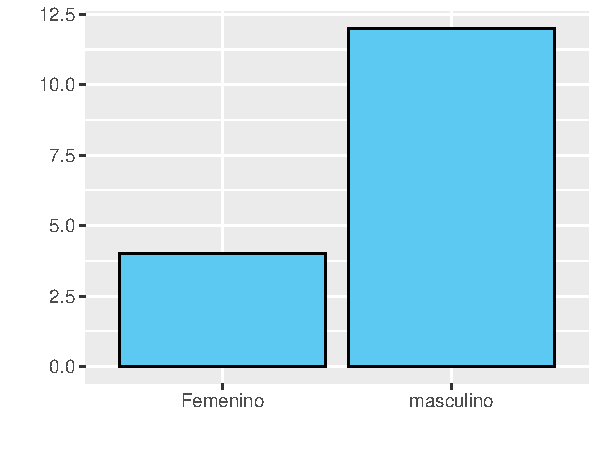
\includegraphics[width=\maxwidth]{figure/uno-1} 
\end{knitrout}
	\caption{Sexo de los encuestados de \comunidad}
	\end{figure}
	Se observa que las cantidades son casi similares, de la cual los de genero masculino es mayor. El alto porcentaje del sexo masculino sugiere que son numerosos en la comunidad de \comunidad en comparación con las mujeres. Esto podría tener varias implicaciones, como patrones de migración de género, roles tradicionales en la sociedad. Sin embargo el porcentaje de las mujeres indican que son una minoría en la sociedad. Finalmente estos datos puden reflejar dinámicas sociales, económicas y culturales particulares en la comunidad de Chilloroya
	\section{Datos generales}
	Edad de los encuestados, de la encuesta realizada se tiene la edad de los participantes, como se muestra a continuacion "mejorar, no redundancia":
	\begin{figure}[H]
	\centering
\begin{knitrout}
\definecolor{shadecolor}{rgb}{0.969, 0.969, 0.969}\color{fgcolor}
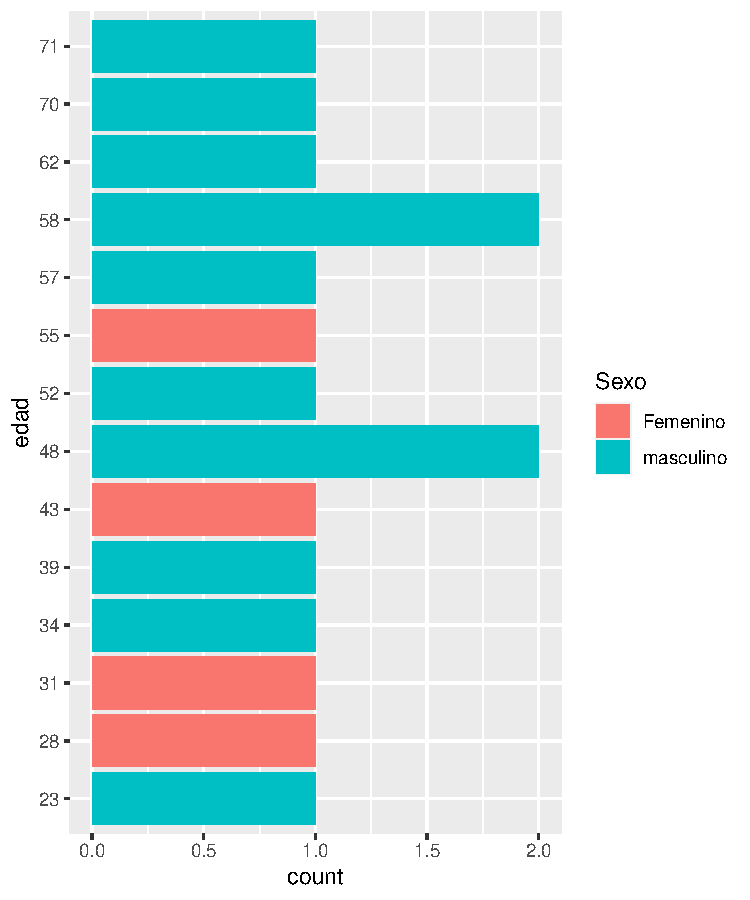
\includegraphics[width=\maxwidth]{figure/dos-1} 
\end{knitrout}
             	
	\caption{Edad de los encuestados de \comunidad}
	\end{figure}
	
Se puede observar que el rango de edades va desde 23 hasta 71 años, siendo las edades de mayor frecuencia el 48 y 58 años los cuales pertenenen al sexo masculino, el alto porcentaje sugiere que la poblacion en estas edades es representativa, esto podría indicar que la comunidad tiene una cantidad significativa de personas adultas lo cual está involucrado en roles de liderazgo, trabajo y toma de decisiones en la \comunidad; asimismo, existen personas entrevistadas de sexo femenino donde la frecuencia es de 43 y 55 años, asimismo se manifiestan en la misma proporción, esto podría sugerir que existen mujeres que tienen capacidad de tomar decisiones en la \comunidad, además existen mujeres Jóvenes de 28 y 31 años en menor cantidad en esta \comunidad, talvez existen factores de migración a otras áreas en busca de educacion o empleo.
	\section{Informacion sobre la vivienda}
Se pregunto respecto a la tenencia de la propiedad en la que habitan los encuestados, de la cual se oberva que el 100\% es propia, como se puede observar en la grafica:
	\begin{figure}[H]
	\centering
\begin{knitrout}
\definecolor{shadecolor}{rgb}{0.969, 0.969, 0.969}\color{fgcolor}
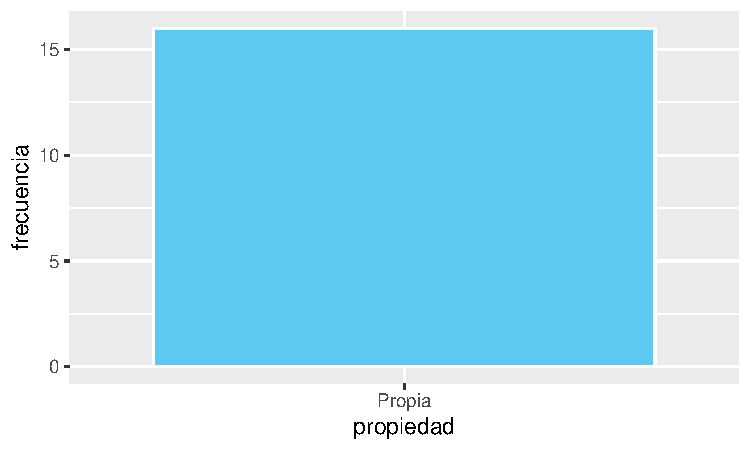
\includegraphics[width=\maxwidth]{figure/tres-1} 
\end{knitrout}
	\caption{Tenencia de la propiedad de los pobladores de \comunidad}
	\end{figure}
	Como se puede observar en el gráfico se tiene que los pobladores de la comunidad de \comunidad tienen casa propia lo que podria indicar una cierta estabilidad en términos de vivienda y posesión de propiedades en la zona. Esto obedece a que las construciones se encuentra inmersa en ecosistemas naturales que conserva, transforma o deteriora.\\
	\\
	Se consulto el tiempo, años, que viven los pobladores en la comunidad, de lo cual se tiene como resultado lo siguiente:
	\begin{figure}[H]
	\centering
\begin{knitrout}
\definecolor{shadecolor}{rgb}{0.969, 0.969, 0.969}\color{fgcolor}
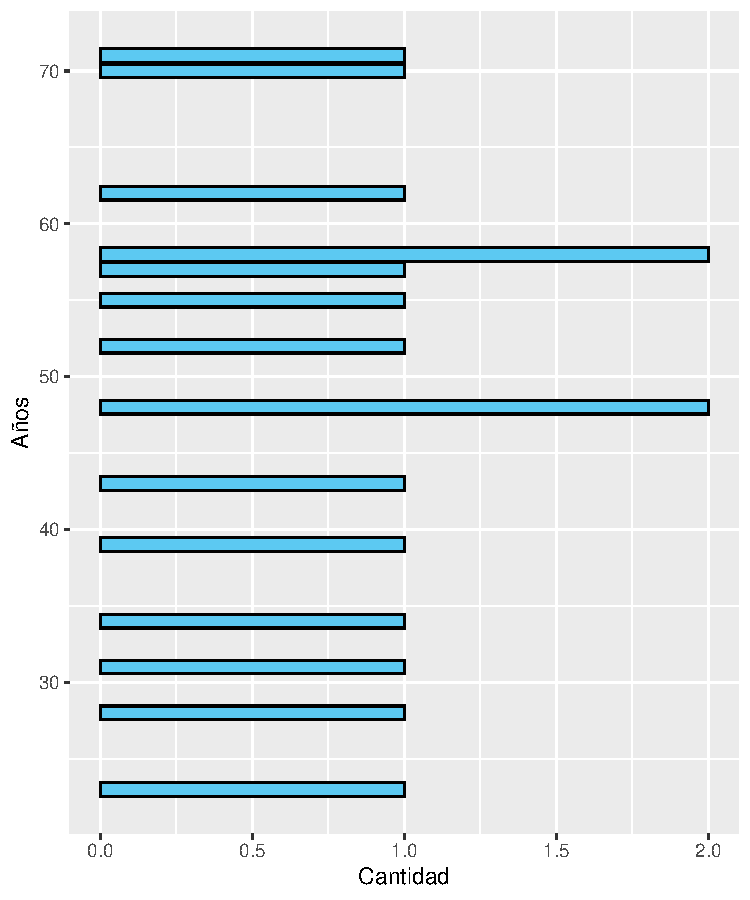
\includegraphics[width=\maxwidth]{figure/cuatro-1} 
\end{knitrout}
	\caption{Años de permanencia de los pobladores en \comunidad}
	\end{figure}
	Se observa que los años que habitan los pobladores van desde 20 a 71, los años que tienen mas frecuencia son de 48 y 58, esto obedece a que los aspectos culturales y ancestrales predominan en la comunidad. Asimismo; estos pobladores son jefes de familia que han heredado costumbres. Finalmente hay personas que habiatan entre 20 a 44 años en la comunidad \\
	\\
	Del idioma que los encuestados se identifico que la todos habla español y quechua, como se grafica:
	\begin{figure}[H]
	\centering
\begin{knitrout}
\definecolor{shadecolor}{rgb}{0.969, 0.969, 0.969}\color{fgcolor}
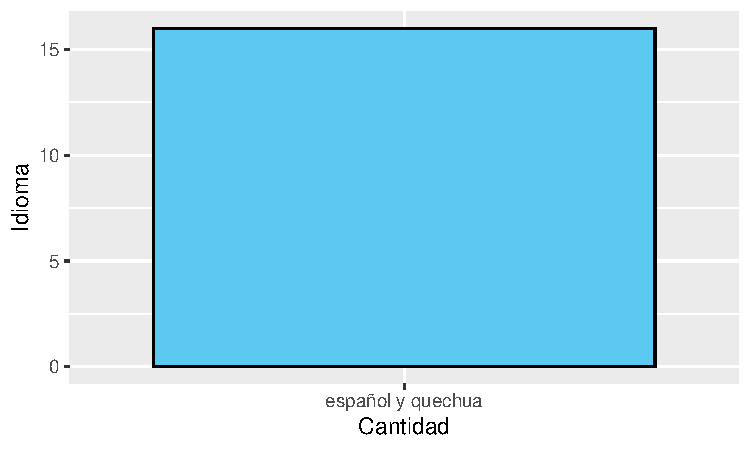
\includegraphics[width=\maxwidth]{figure/cinco-1} 
\end{knitrout}
	\caption{Idioma que habla el poblador}
	\end{figure}
	Se observa que el total de los encuestados hablan español y quechua. Esto explica que los pobladores de la comunidad de \comunidad son bilingües, esto sugiere que la educación en la comunidad marcó un hito importante en la lengua, donde se intercambi quechua fortalece nuestra identidad nacional,  "mejorar".
	\section{Informacion de servicios}
	De la fuente de agua que los pobladores se abastecen se identifico lo siguiente:
	\begin{figure}[H]
	\centering
\begin{knitrout}
\definecolor{shadecolor}{rgb}{0.969, 0.969, 0.969}\color{fgcolor}
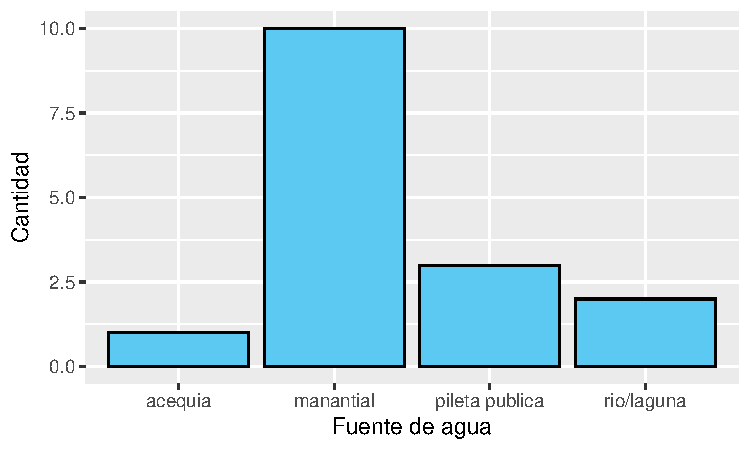
\includegraphics[width=\maxwidth]{figure/seis-1} 
\end{knitrout}
	\caption{Fuente de agua para consumo de agua de los pobladores de \comunidad}
	\end{figure}
	La fuente de manantial es la mas usada por los pobladores de la comunida de \comunidad las cuales tienen un origen subterraneo que emergen espontanemente en la superfcie. Seguido del abastecimeinto de pileta pública donde son controlados por los directivos de las juntas administradoras de servicios de saneamiento (JASS), esto quiere decir que la población de la mencionado comunidad realizan actividades de limpieza y desinfección, en consecuencia tambien consumen agua proveniente de rio o laguna, finalmente hay un pequeño grupo que se abastece de agua de las acequias.\\
	\\
	La eliminacion de basura en las viviendas de los pobladores es la siguiente
	\begin{figure}[H]
	\centering
\begin{knitrout}
\definecolor{shadecolor}{rgb}{0.969, 0.969, 0.969}\color{fgcolor}
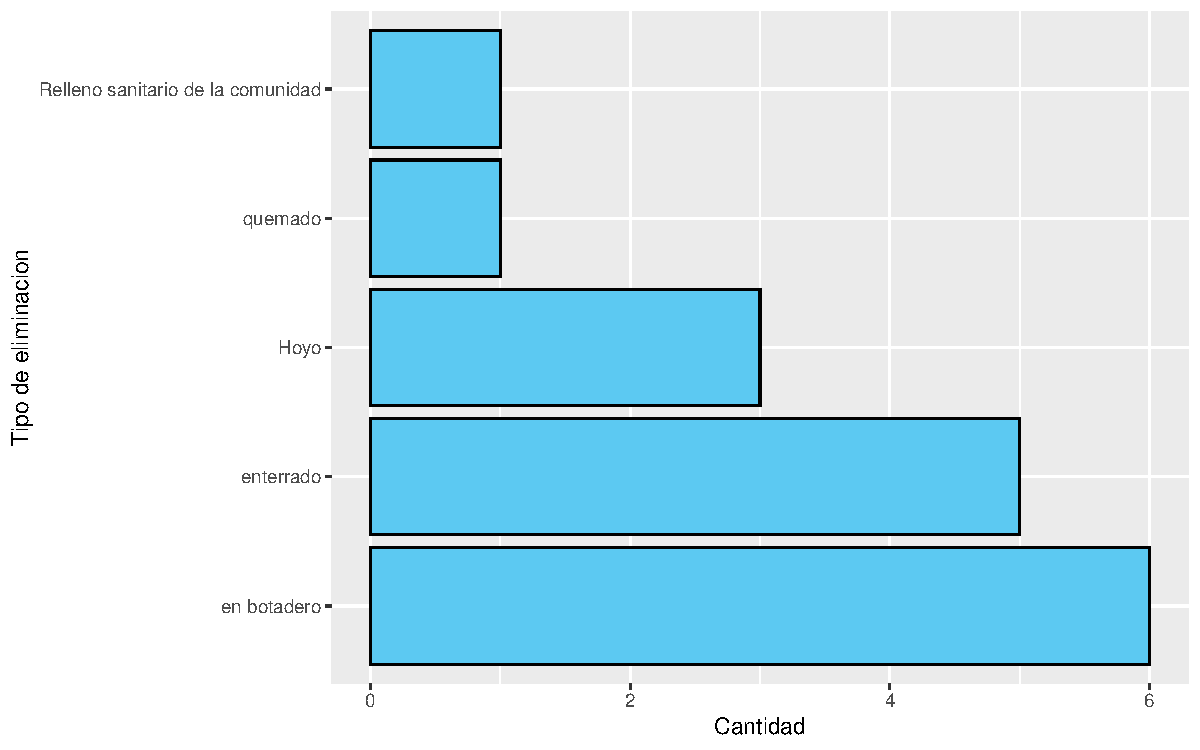
\includegraphics[width=\maxwidth]{figure/siete-1} 
\end{knitrout}
	\caption{Eliminacion de la basura en \comunidad}
	\end{figure}
	Los tipos de eliminacion con mayor frecuencia es el botadero. Esto sugiere que existe una organización de los pobladores y de las instituciones que intervinene en el cuidado del medio ambiente, además se precisa que existen pobladores que entierran los desechos para propiciar la descomposición de la basura, tambien se observa que hay comuneros que realizan el hoyo para almacenar la basura, un pequeño grupo realiza la actividad del quemado, finalmente un porcentaje minoritario usa el relleno sanitario de la comunidad.\\
	\\
	Para la preparacion de sus alimentos las personas utilizan los siguientes combustibles:
	\begin{figure}[H]
	\centering
\begin{knitrout}
\definecolor{shadecolor}{rgb}{0.969, 0.969, 0.969}\color{fgcolor}
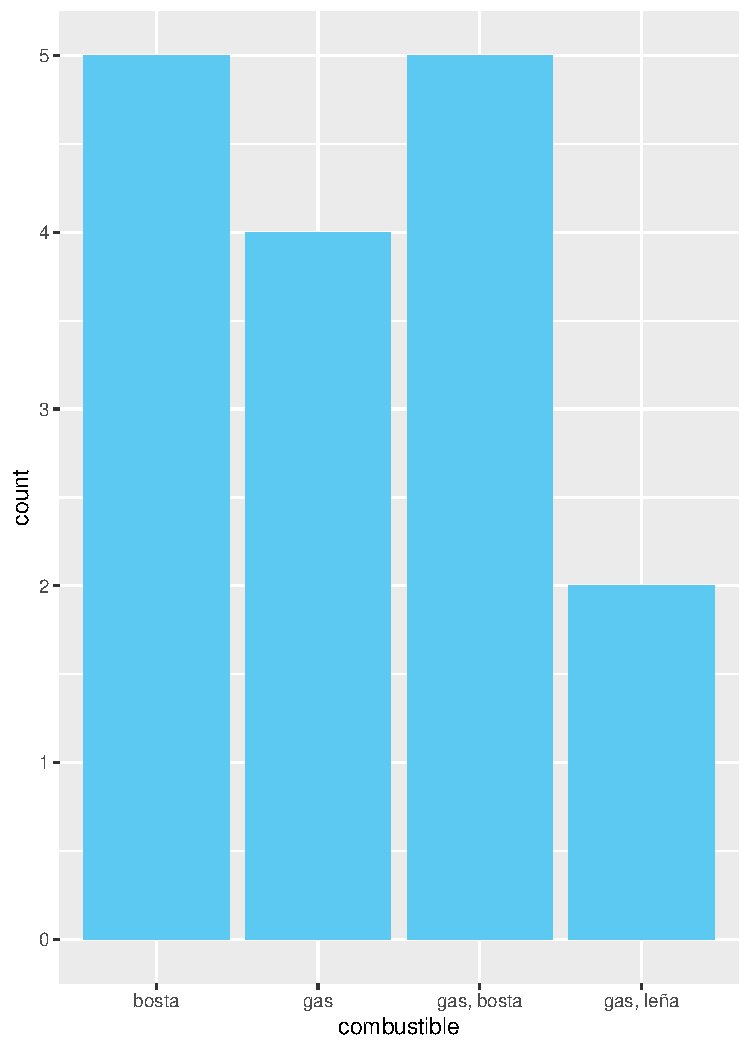
\includegraphics[width=\maxwidth]{figure/ocho-1} 
\end{knitrout}
	\caption{Uso de combustible para preparacion de alimentos en \comunidad}
	\end{figure}
	Los pobladores usan con mas frecuencia bosta y bosta y gas, los habitantes aprovechan el estiercol del ganado para preparar alimentos en lugares donde es muy complicado conseguir leña de madera asimismo el Gas es utilizado por la familias en la comunidad de \comunidad, esto sugiere que el poder de adquisicion de este elemento se ha incrementado en el consumo, dado que se les hace mas accesible con respecto al precio, el gobierno destina un descuento exclusivo mediante fondo de inclusion Social Energético (FISE) esto se llama compensacion social y acceso a GLP. Existe una pequeña proporcion de familias que usan gas y leña al mismo tiempo. Cabe mencionar que la población usa el Gas cuando el bosta y leña no están en cponsiciones adecuadas o están en temporadas de iniverno la cual se les hace muy complicado preprarar los alimentos.\\
	\\
	Las enfermedades que mas aquejan a la poblacion son las siguientes:
	\begin{figure}[H]
	\centering
\begin{knitrout}
\definecolor{shadecolor}{rgb}{0.969, 0.969, 0.969}\color{fgcolor}
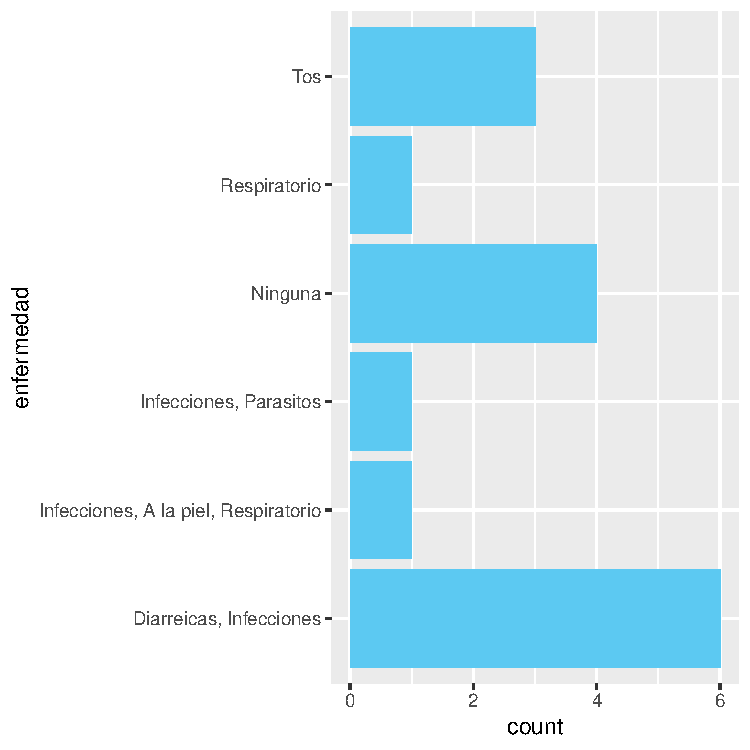
\includegraphics[width=\maxwidth]{figure/nueve-1} 
\end{knitrout}
	\caption{Enfermedades que aquejan a los pobladores de \comunidad}
	\end{figure}
	Se observa en el gráfico que las enfermedades que mas aqueja a las familias de la comunidad de \comunidad son las enfermedades diarreicas e infecciones, esto sugiere que la falta de higiene, la ingestión del agua y alimentos contaminados son las vías por medio de las cuales se adquieren estos malestares. Seguido de un porcentaje predominante señalan que no tienen ningna enfermedad.\\
	\\
	Además se oberva que existen familias que tienen tos, esto afirma que la altitud del lugar influye en la salud de las personas, además la causa mas frecuente respecto a este mal es la enfermedad pulmonar obstructiva, generalmente este caso afecta a los niños y personas que se encuentran en la tercera edad.Finalmente se tiene las enfermedades que mas afecta a la población son la Infecciones a la piel, infecciones y problemas respiratorios en la misma proporción.\\
	\\
	Las personas que sufren de alguna enfermedad se atienden en los siguientes lugares:
	\begin{figure}[H]
	\centering
\begin{knitrout}
\definecolor{shadecolor}{rgb}{0.969, 0.969, 0.969}\color{fgcolor}
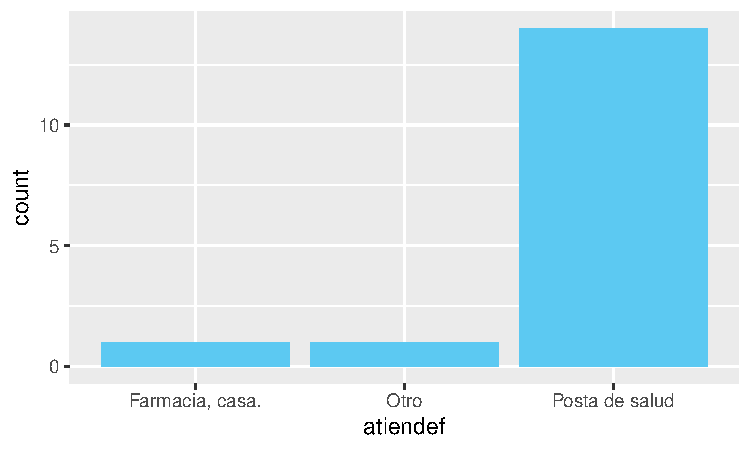
\includegraphics[width=\maxwidth]{figure/once-1} 
\end{knitrout}
	\caption{Lugar de atencion cuando se enferman}
	\end{figure}
  Los datos de la gráfica muestran que los pobladores de la comunidad de \comunidad acuden a la posta de salud mas cercana, esto indica que estos establecimientos de salud son actores esenciales que atienden emergencias o contingencias en el lugar. Seguido de un pequeño grupo de familias que acuden a las farmacias  de manera periódica en la capital de distrito, además hay pobladores que remedian sus enfermedades en su vivienda con tratamientos caseros.\\
  \\
	Se consulto si estas personas cuentan con seguro medico, de lo cual se obtuvo el siguiente resultado:
	\begin{figure}[H]
	\centering
\begin{knitrout}
\definecolor{shadecolor}{rgb}{0.969, 0.969, 0.969}\color{fgcolor}
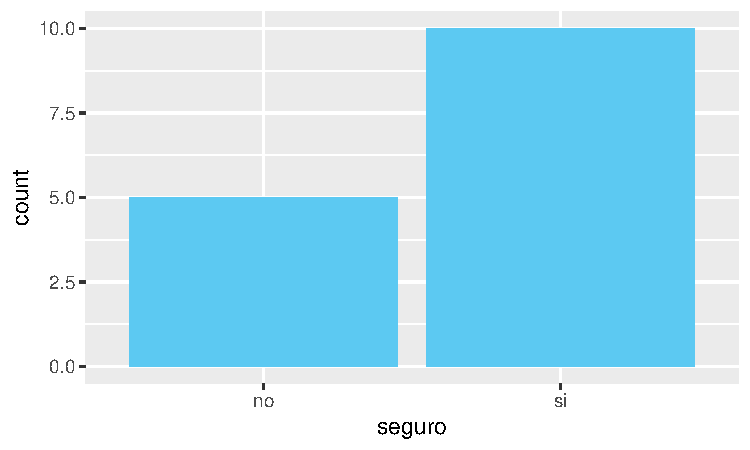
\includegraphics[width=\maxwidth]{figure/doce-1} 
\end{knitrout}
	\caption{Uso de un seguro medico}
	\end{figure}
	Los resultados de este gráfico indican que sí cuentan con seguro médico, esto podría sugerir que la población desde su nacimiento tiene derecho a la salud o al Seguro Integral de Salud(SIS), asimismo existen personas que cuentan con seguros ya sea privado o Essalud. Seguido de un pequeño porcentaje de pobladores que no tienen seguro de salud, esto indica que perdieron el SIS por que han ingresado a otro seguro de manera temporal o la misma población migra a otras comunidades o ciudades lo cual dificulta que puedan acceder a un seguro.\\
	\\
	Se consulto respecto a la preferencia de emisoras radiales que se escucha, al respecto se tiene como primera emisora de preferencia la siguiente:
	\begin{figure}[H]
	\centering
\begin{knitrout}
\definecolor{shadecolor}{rgb}{0.969, 0.969, 0.969}\color{fgcolor}
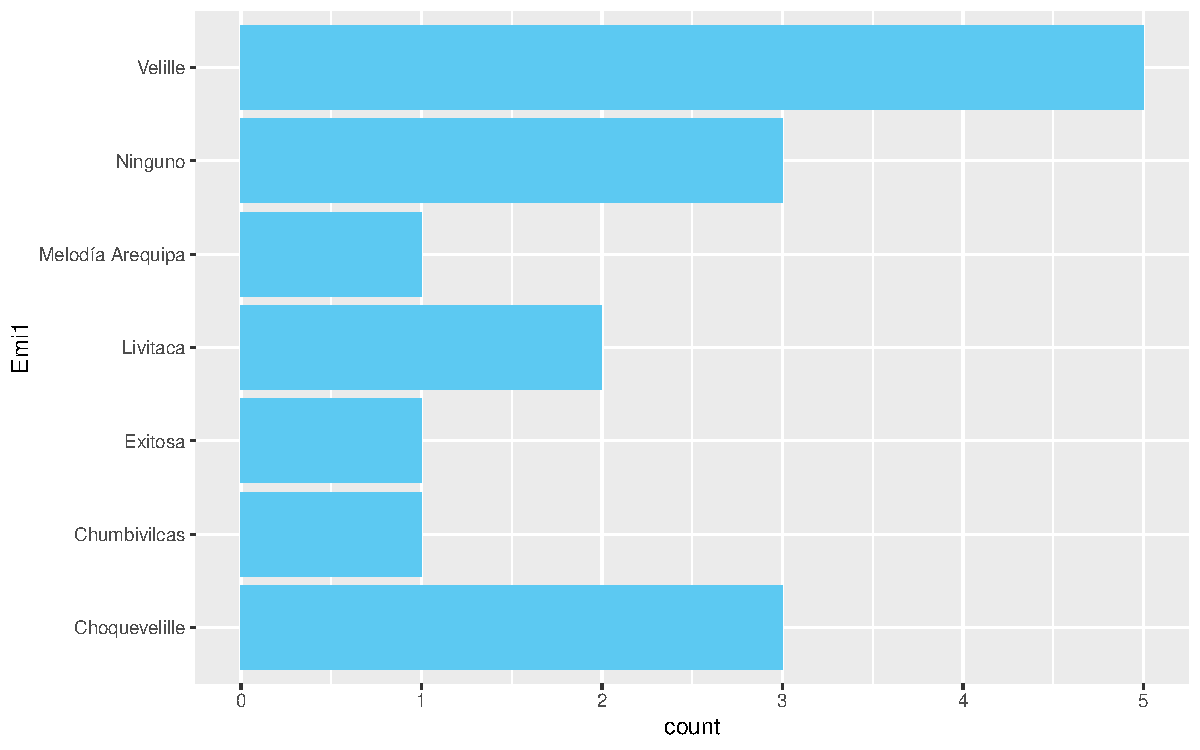
\includegraphics[width=\maxwidth]{figure/one-1} 
\end{knitrout}
	\caption{Primera emisora que se escucha}
	\end{figure}
	Como se puede observar la emisora con mayor audiencia es Velille, seguido de emisora Choquevelille, ademá existe un porcentaje de la población que no tiene preferencia radial. Un grupo de familias Sintoniza Radio Livitaca, seguido de un grupo limitado escuchan radio Melodía Arequipa, Exitosa y Chumbivilcas respectimanete.\\
	\\
	El horario que los encuestados prefieren escuchar es el siguiente:
	\begin{figure}[H]
	\centering
\begin{knitrout}
\definecolor{shadecolor}{rgb}{0.969, 0.969, 0.969}\color{fgcolor}
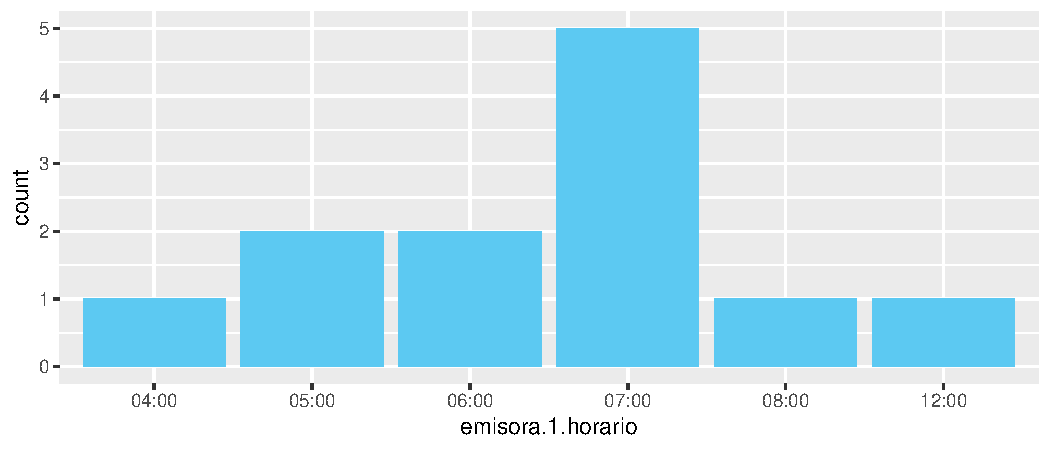
\includegraphics[width=\maxwidth]{figure/two-1} 
\end{knitrout}
	\caption{Horario de emisora preferida}
	\end{figure}
	Los datos de la gráfica señalan que el horario habitual que sintonizan la radio en la \comunidad es a las 7:00 a.m. Además existen familias que encienden la radio a las 5:00 a.m. y 6:00 de la mañana, tambien hay un horario de 8:00 y 12:00 del medio día que prefieren escuchar la radio. Finalmente un grupo reducido de personas sintonizan a las 4:00 de la madrugada.\\
	\\
Emisoras y horarios preferidos:
	\begin{figure}[H]
	\centering
\begin{knitrout}
\definecolor{shadecolor}{rgb}{0.969, 0.969, 0.969}\color{fgcolor}
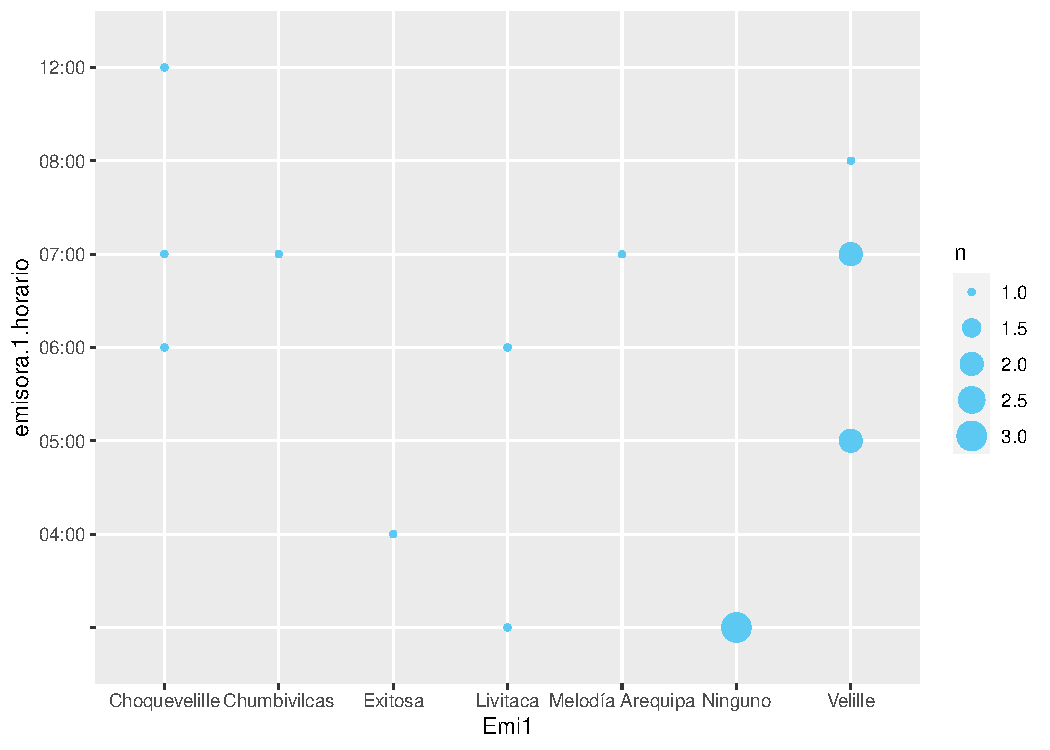
\includegraphics[width=\maxwidth]{figure/three-1} 
\end{knitrout}
	\caption{Emisoras y horarios preferidos}
	\end{figure}
	Como se muestra en el gráfico los horarios preferidos  que sintonizan en la comunidad de \comunidad es a las 7:00 a.m. lo cual es escuchada por 2 personas, hay solo una persona que enciende la radio en los horarios de 4:00, 6:00, 8:00 y 12:00 del meridiano.\\ 
	\\
	
	Se consulto respecto a la preferencia de emisoras radiales que se escucha, al respecto se tiene como primera emisora de preferencia la siguiente:
	\begin{figure}[H]
	\centering
\begin{knitrout}
\definecolor{shadecolor}{rgb}{0.969, 0.969, 0.969}\color{fgcolor}
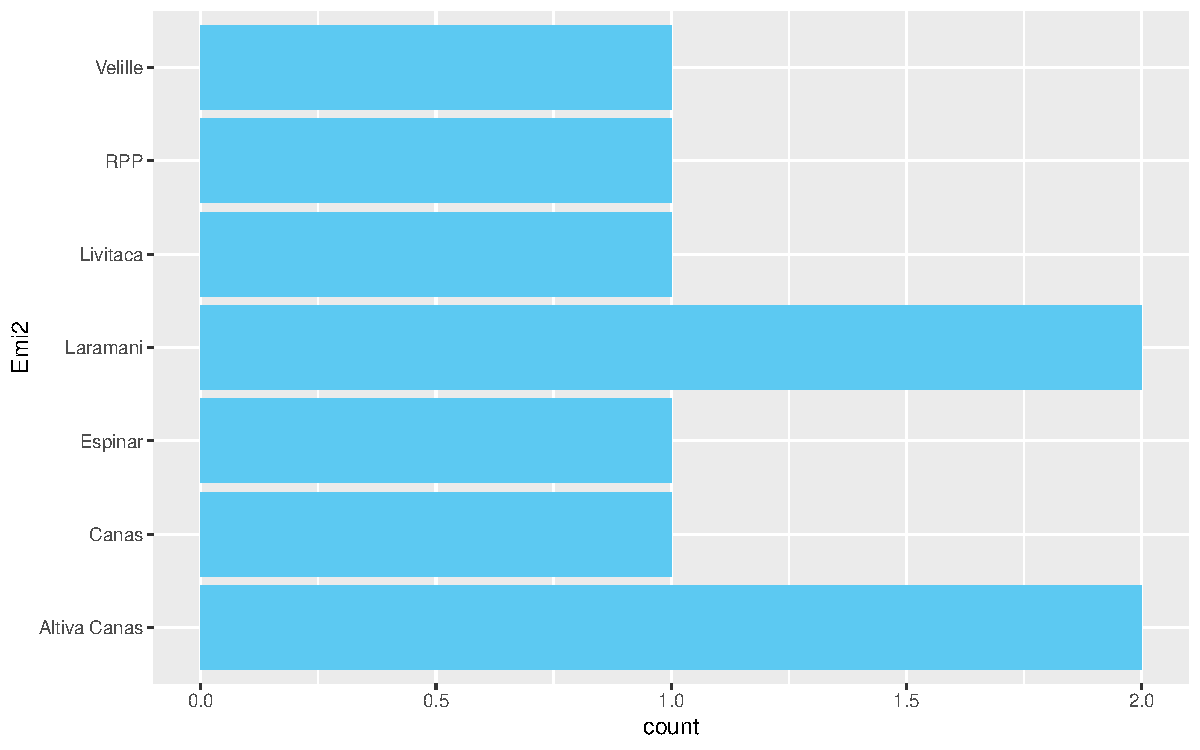
\includegraphics[width=\maxwidth]{figure/four-1} 
\end{knitrout}
	\caption{Seguna emisora que se escucha}
	\end{figure}
	De la primera emisora que mas se escucha en la comunidad de \comunidad se identificó que la radio Laramani y Altiva Canas son de mayor preferencia por los pobladores de la zona; sin embargo las emisoras radiales Canas, Espinar, Livitaca, RPP y Velille tienen una menor preferencia.\\
	\\
	El horario que los encuestados prefieren escuchar es el siguiente:
	\begin{figure}[H]
	\centering
\begin{knitrout}
\definecolor{shadecolor}{rgb}{0.969, 0.969, 0.969}\color{fgcolor}
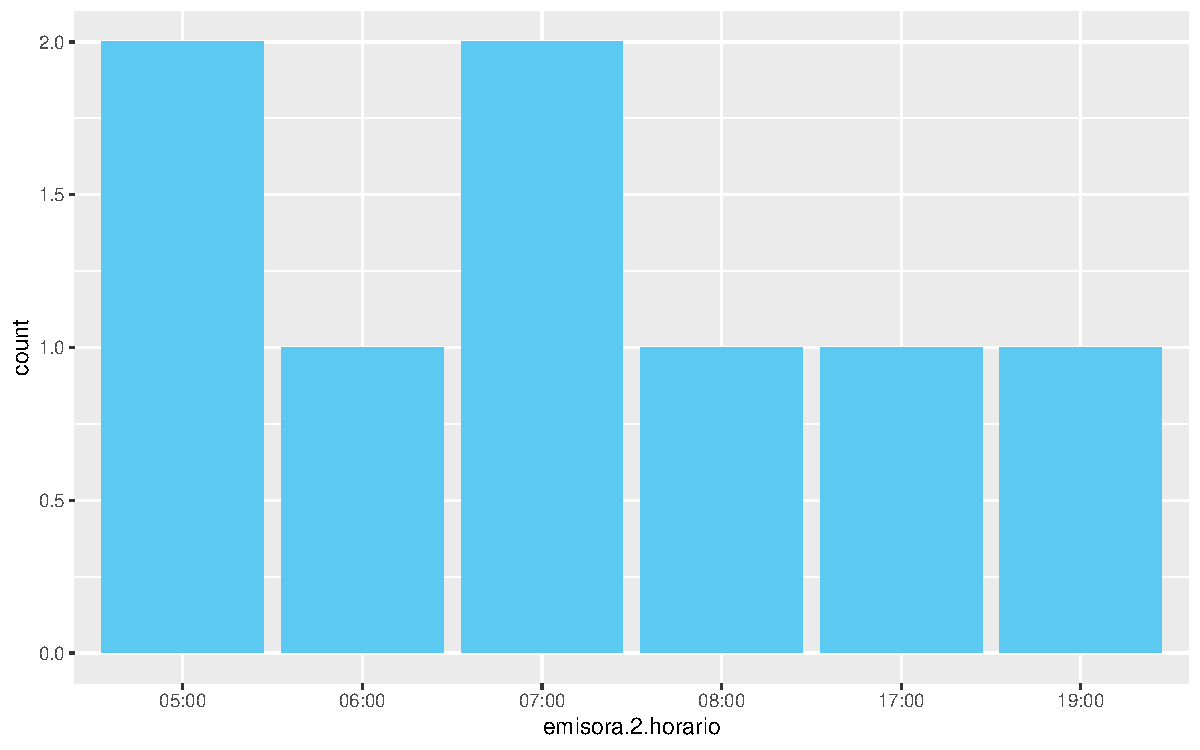
\includegraphics[width=\maxwidth]{figure/five-1} 
\end{knitrout}
	\caption{Horario de emisora preferida}
	\end{figure}
	Los datos de la gráfica muestran que los encuestados tienen una preferencia de escuchar la radio como como segunda opción en el horario de 5:00 y 7:00 de la mañana; finalmente, e oberva que exiten familias que prefieren escuchar en los horarios de 6:00, 8:00 de la mañana y 17:00 y 19:00 de la noche proporcionalmente.\\
	\\
	Emisora y horarios preferidos: 
	\begin{figure}[H]
	\centering
\begin{knitrout}
\definecolor{shadecolor}{rgb}{0.969, 0.969, 0.969}\color{fgcolor}
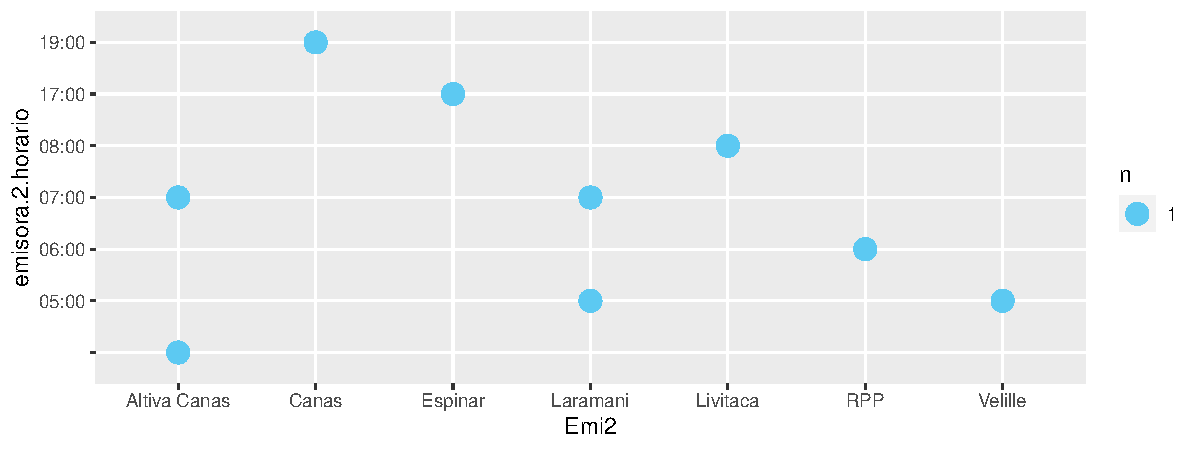
\includegraphics[width=\maxwidth]{figure/six-1} 
\end{knitrout}
	\caption{Emisoras y horarios preferidos}
	\end{figure}
	Se observa tambien en este gráfico que el horario preferido para escuchar la segunda emisora es a las 7:00 y 5:00 de la mañana; asimismo, hay pobladores que sintonizan en el horario de 6:00 y 8:00 a.m. finalmente hay familias que encienden la radio en el horario de la noche las cuales son 17:00 p.m.  19:00 p.m.
	
	
	\section{Datos agropecuarios}
	De la actividad agropecuaria, se pregunto que cultivos como primera opcion realizan, de lo cual se obtuvo la siguiente informacion:
	\begin{figure}[H]
	\centering
\begin{knitrout}
\definecolor{shadecolor}{rgb}{0.969, 0.969, 0.969}\color{fgcolor}
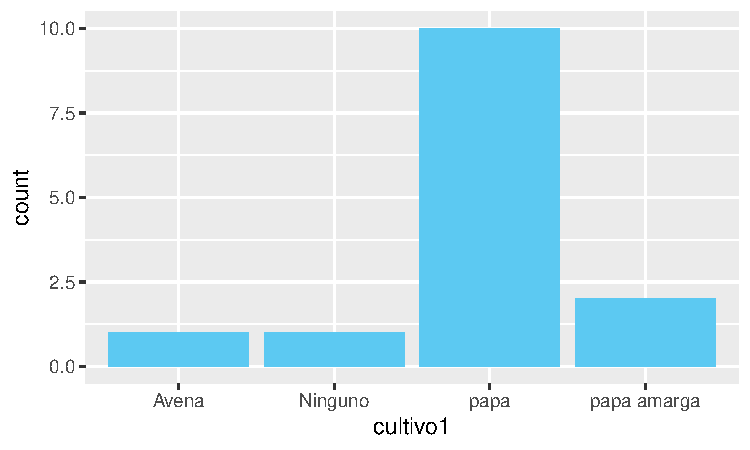
\includegraphics[width=\maxwidth]{figure/seven-1} 
\end{knitrout}
	\caption{Cultivo al que se dedican las personas}
	\end{figure}
	En la comunidad de \comunidad se tiene que el producto que mas se cultiva es la papa en gran proporción, esto sugiere que este tubérculo se ha convertido en un notable impulsor de la economía de la comunidad tal como señalan, asu ves dota de mayores ingresos a las familias, además un pequeño porcentaje cultiva papa amarga que generalmente lo extraen de las partes altas del lugar. Tambien se puede observar que cultivan Avena en menor proporción, lo cual podría indicar que es de autoconsumo o simplemente sirve para alimentar a los animales de casa, finalmete se pudo ver que hay familias que no se dedican a la actividad agrícola.\\
	\\
	De la cantidad de cultivo se tiene lo siguiente:
	\begin{figure}[H]
	\centering
\begin{knitrout}
\definecolor{shadecolor}{rgb}{0.969, 0.969, 0.969}\color{fgcolor}
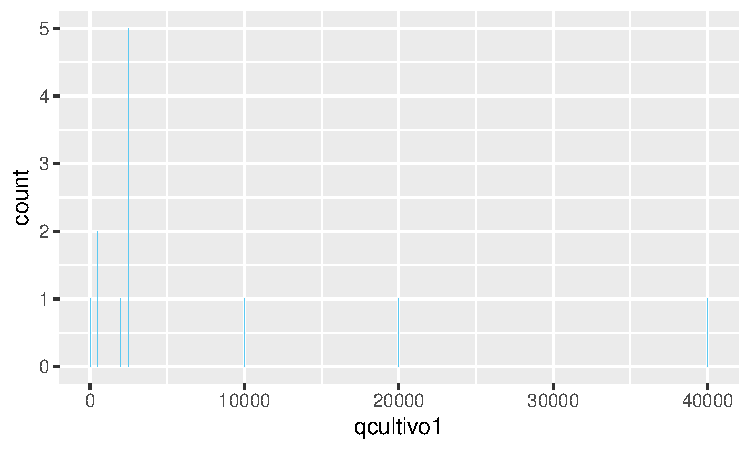
\includegraphics[width=\maxwidth]{figure/eight-1} 
\end{knitrout}
	\caption{Primera opcion de cultivo en \comunidad \- en cantidades}
	\end{figure}
	
	De los datos del gráfico se puede observar que de las personas encuestadas cultivan papa  en una cantidad de 4000 kilos, seguido de la papa amarga donde 2 personas cultivan 2500 kilos, asu ves una persona  encuestada cultiva 1500 Kg de avena.\\
	\\
	Cantidad de cultivo por producto:
	\begin{figure}[H]
	\centering
\begin{knitrout}
\definecolor{shadecolor}{rgb}{0.969, 0.969, 0.969}\color{fgcolor}
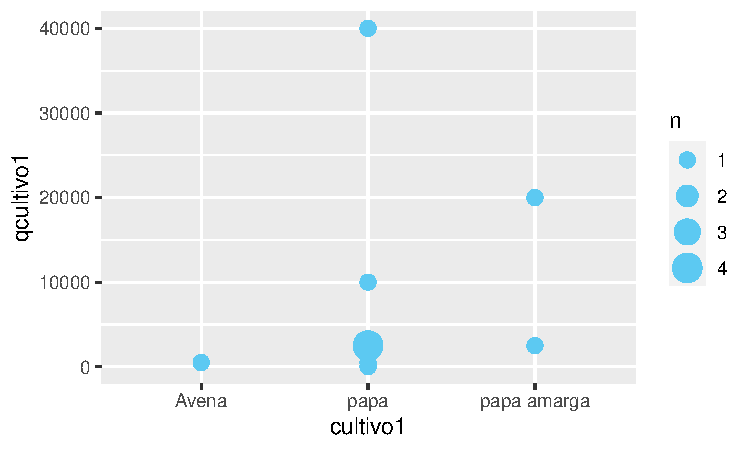
\includegraphics[width=\maxwidth]{figure/oneh-1} 
\end{knitrout}
	\caption{Cantidad de cultivo por producto}
	\end{figure}
	El gráfico muestra la cantidad de cultivo por producto, dode se aprecia que la producción de la papa es de 40000 kilos en la comunidad de \comunidad, seguido de la papa amarga lo cual se produce en 2500 kilos y finalmente la avena que tiene una producción 1971 kilos.\\
	\\
	Método de cultivo de primera opción:
	\begin{figure}[H]
	\centering
\begin{knitrout}
\definecolor{shadecolor}{rgb}{0.969, 0.969, 0.969}\color{fgcolor}
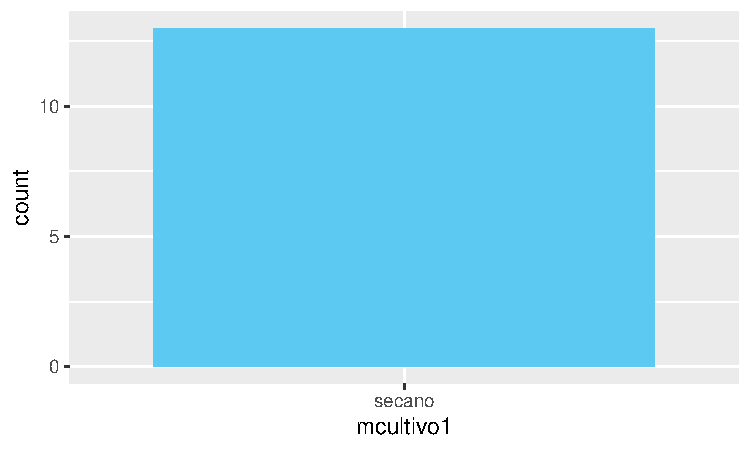
\includegraphics[width=\maxwidth]{figure/twelve-1} 
\end{knitrout}
	\caption{Metodo de cultivo de la primera opcion de cultivo}
	\end{figure}
	El dato del gráfico muestra que el secano es el primer método como opción en la \comunidad, cabe señalar que existe el agua de la lluvia donde propicia la producción natural.\\
	\\
	De la actividad agropecuaria, se pregunto que cultivos como segunda opcion realizan, de lo cual se obtuvo la siguiente informacion:
	\begin{figure}[H]
	\centering
\begin{knitrout}
\definecolor{shadecolor}{rgb}{0.969, 0.969, 0.969}\color{fgcolor}
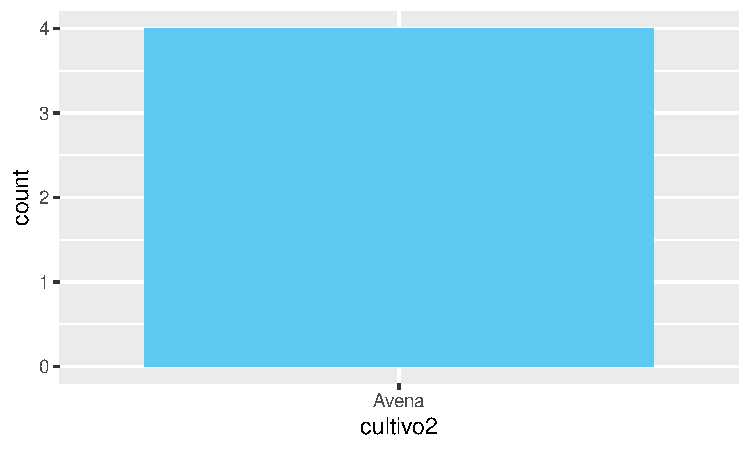
\includegraphics[width=\maxwidth]{figure/nine-1} 
\end{knitrout}
	\caption{Cultivo al que se dedican las personas como segunda opcion}
	\end{figure}
	Se observa que el cultivo de avena es la segunda opción mas rentable en la produccion por parte de las personas en la \comunidad.\\
	\\
	De la cantidad de cultivo se tiene lo siguiente:
	\begin{figure}[H]
	\centering
\begin{knitrout}
\definecolor{shadecolor}{rgb}{0.969, 0.969, 0.969}\color{fgcolor}
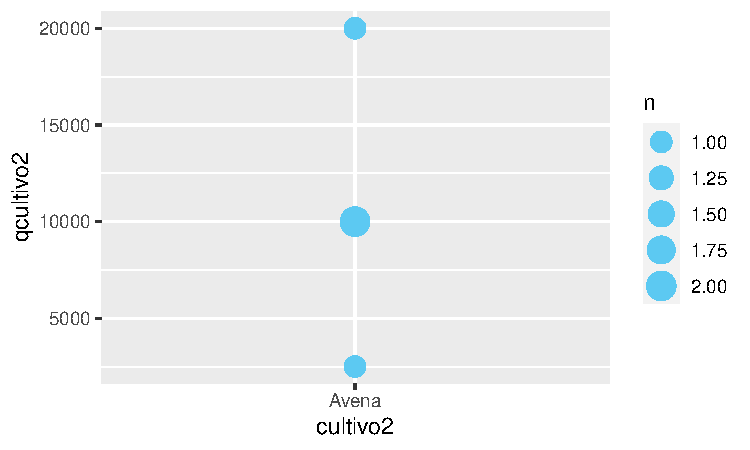
\includegraphics[width=\maxwidth]{figure/ten-1} 
\end{knitrout}
	\caption{Cantidad de cultivo de la segunda opcion de cultivo en \comunidad}
	\end{figure}
	El dato del gráfico afirma que la produccion de la avena en la comunidad de Chilloroya asciende a los 10000 kilos. como segunda opción de cultivo\\
	\\
	Método de cultivo de la segunda opción:
	\begin{figure}[H]
	\centering
\begin{knitrout}
\definecolor{shadecolor}{rgb}{0.969, 0.969, 0.969}\color{fgcolor}
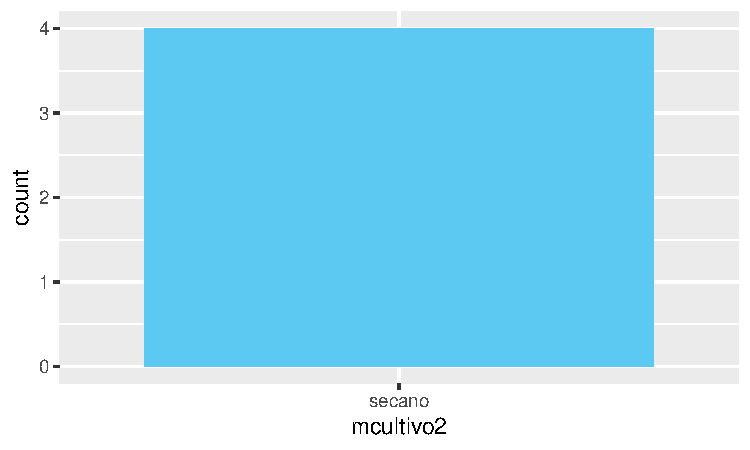
\includegraphics[width=\maxwidth]{figure/eleven-1} 
\end{knitrout}
	\caption{Metodo de cultivo de la segunda opcion de cultivo en \comunidad}
	\end{figure}
	El dato del gráfico indica que el método de cultivo de la segunda opción(avena)en la \comunidad es el secano, sugiere que la población usa el agua de la lluvia mas no de otras fuentes de abastecimientos de agua para la producción.\\
	\\
	
	De la actividad agropecuaria, se pregunto que cultivos como tercera opcion realizan, de lo cual se obtuvo la siguiente informacion:
	\begin{figure}[H]
	\centering
\begin{knitrout}
\definecolor{shadecolor}{rgb}{0.969, 0.969, 0.969}\color{fgcolor}
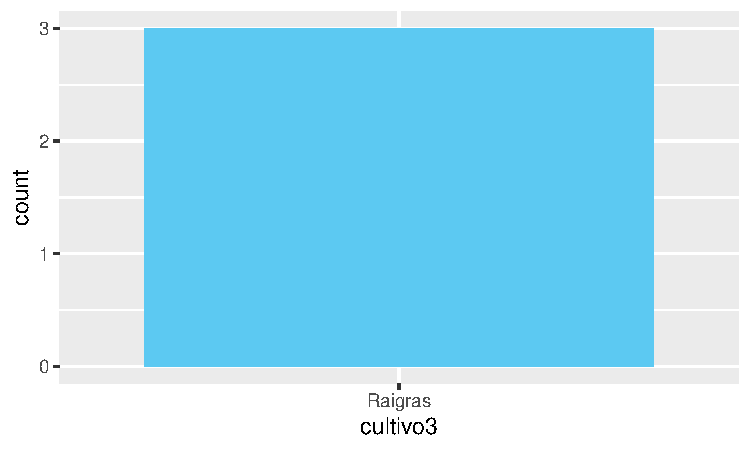
\includegraphics[width=\maxwidth]{figure/thirteen-1} 
\end{knitrout}
	\caption{Cultivo al que se dedican las personas como tercera opcion}
	\end{figure}
	Se observa que el cultivo que a la que las personas se dedican como tercera opción es Rye grass. Lo cual podría cocluir que este producto sirve para alimentar a las ovejas, caballos y terneras de recría en la comunidad, tambien podría indiacar que es una energía metabolizable para los animales\\
	\\
	De la cantidad de cultivo se tiene lo siguiente:
	\begin{figure}[H]
	\centering
\begin{knitrout}
\definecolor{shadecolor}{rgb}{0.969, 0.969, 0.969}\color{fgcolor}
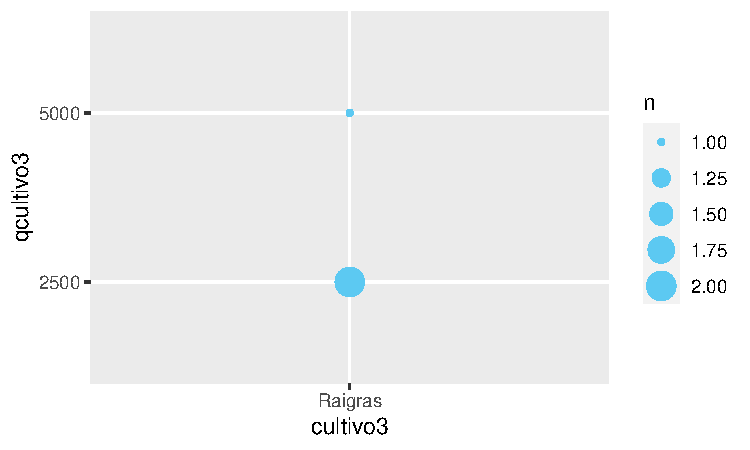
\includegraphics[width=\maxwidth]{figure/fourteen-1} 
\end{knitrout}
	\caption{Cantidad de cultivo de la tercera opcion de cultivo en \comunidad}
	\end{figure}
	Se evidencia que la cantidad  de produccion de cultivo como tercera opción es la Rye Grass donde llega a los 5000 kilos en la comunidad de Chilloroya.\\
	\\
	
	
	De la actividad agropecuaria, se pregunto que animales cria segunda opcion, de lo cual se obtuvo la siguiente informacion:
	\begin{figure}[H]
	\centering
\begin{knitrout}
\definecolor{shadecolor}{rgb}{0.969, 0.969, 0.969}\color{fgcolor}
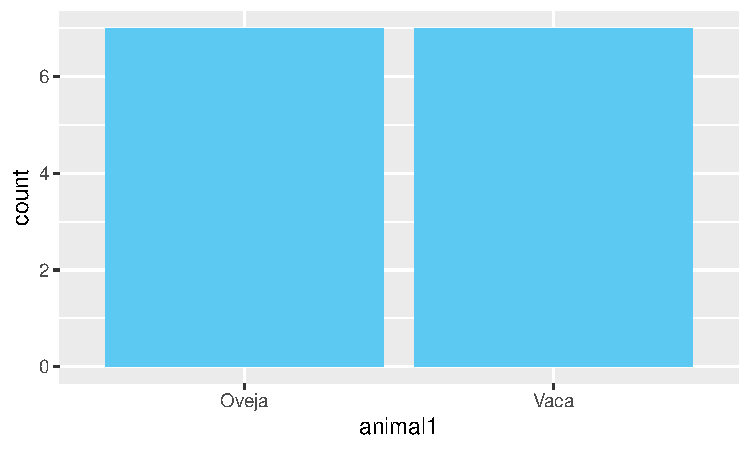
\includegraphics[width=\maxwidth]{figure/fifteen-1} 
\end{knitrout}
	\caption{Animales al que se dedican las personas como primera opcion}
	\end{figure}
	Del gráfico se concluye que la crianza a la que las personas se dedican como primera opción es la Oveja y Vaca. Esto podría indicar que la economía de la comunidad de Chilloroya depende en gran medida de estos ovinos; asimismo podrían aprovechar la lana, Carne, leche, cuero y estircol.\\
	\\
	De la cantidad de animales que crian se tiene lo siguiente:
	\begin{figure}[H]
	\centering
\begin{knitrout}
\definecolor{shadecolor}{rgb}{0.969, 0.969, 0.969}\color{fgcolor}
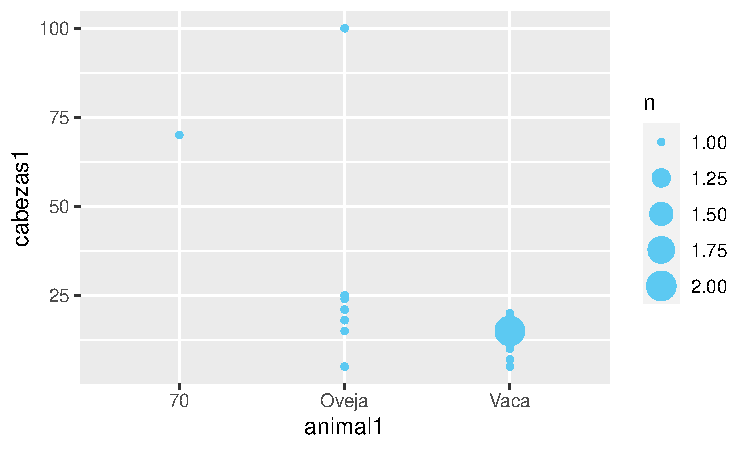
\includegraphics[width=\maxwidth]{figure/sixteen-1} 
\end{knitrout}
	\caption{Cantidad de animales criados de primera opcion en funcion a la cantidad y especie en \comunidad}
	\end{figure}
	Los datos del gráfico señalan que en promedio las familias tienen en su poder 100 ovejas, asimismo tienen vacas que se comportan en una mínima cantidad de 22 cabezas.\\
	\\
	Método de crianza de la primera opción: 
	\begin{figure}[H]
	\centering
\begin{knitrout}
\definecolor{shadecolor}{rgb}{0.969, 0.969, 0.969}\color{fgcolor}
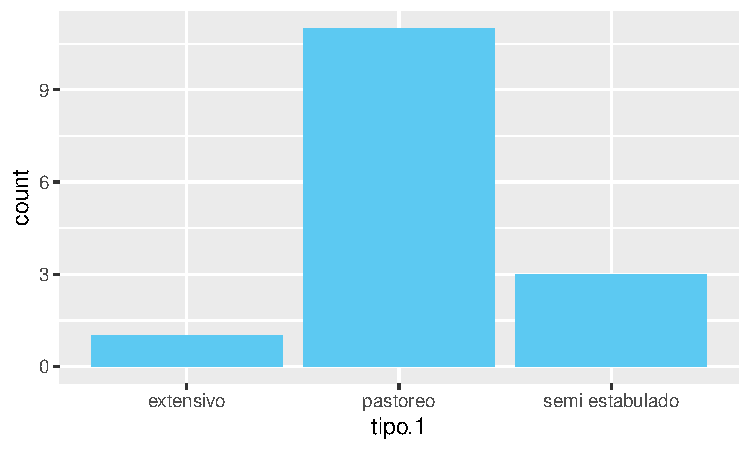
\includegraphics[width=\maxwidth]{figure/seventeen-1} 
\end{knitrout}
	\caption{Metodo de crianza de la primera opcion de crianza de animales en \comunidad}
	\end{figure}
	Los datos de la gráfica indican que el método de crianza de primera opción es el pastoreo, seguidodel método del semi estabulado y finalmente el extensivo\\
	\\
	
	De la actividad agropecuaria, se pregunto que animales cria como segunda opción, de lo cual se obtuvo la siguiente informacion:
	\begin{figure}[H]
	\centering
\begin{knitrout}
\definecolor{shadecolor}{rgb}{0.969, 0.969, 0.969}\color{fgcolor}
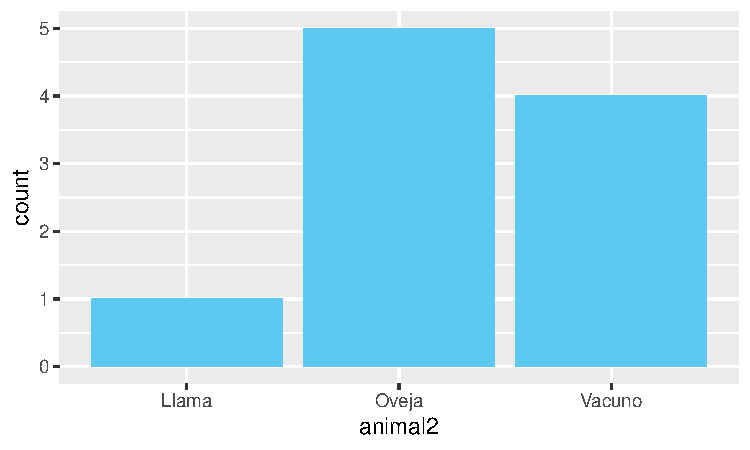
\includegraphics[width=\maxwidth]{figure/eighteen-1} 
\end{knitrout}
	\caption{Animales al que se dedican las personas como segunda opcion}
	\end{figure}
	Los datos del gráfico muestran que las familias crian como segunda opción en gran proporción a la oveja , lo cual supera a la crianza del vacuno y Llama.\\
	\\
	De la cantidad de animales que crian se tiene lo siguiente:
	\begin{figure}[H]
	\centering
\begin{knitrout}
\definecolor{shadecolor}{rgb}{0.969, 0.969, 0.969}\color{fgcolor}
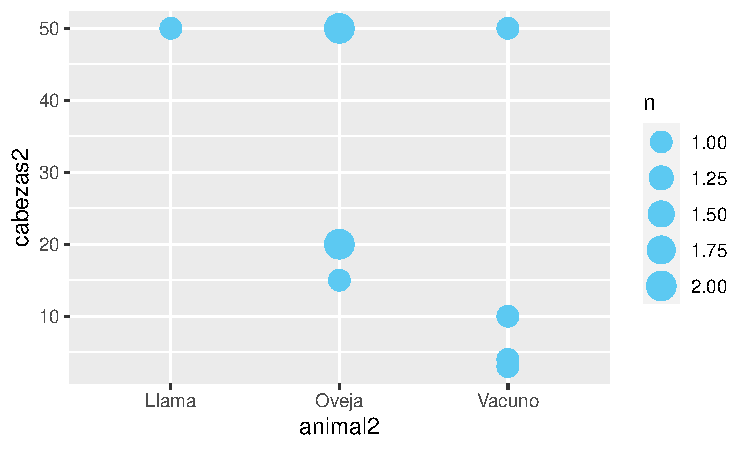
\includegraphics[width=\maxwidth]{figure/nineteen-1} 
\end{knitrout}
	\caption{Cantidad de animales criados de segunda opcion en funcion a la cantidad y especie en \comunidad}
	\end{figure}
	Del gráfico se puede concluir que existen 50 cabezas entre ovejas, vacunos y llamas en crianza como segunda opción\\
	\\ 
	Método de crianza de la segunda opoción:
	\begin{figure}[H]
	\centering
\begin{knitrout}
\definecolor{shadecolor}{rgb}{0.969, 0.969, 0.969}\color{fgcolor}
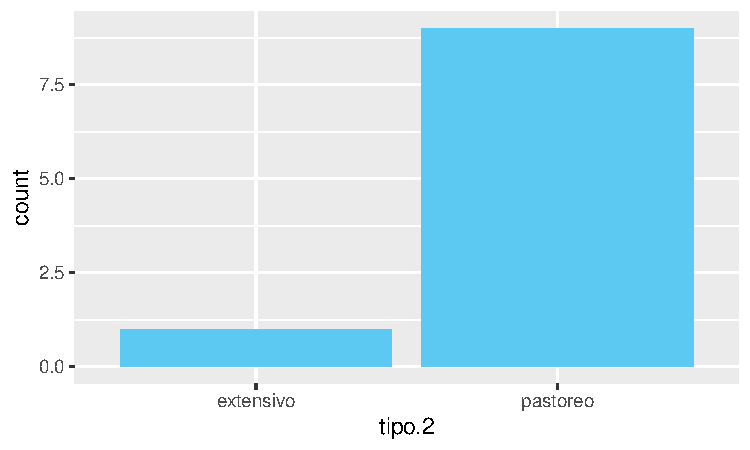
\includegraphics[width=\maxwidth]{figure/twenty-1} 
\end{knitrout}
	\caption{Metodo de crianza de la segunda opcion de crianza de animales en \comunidad}
	\end{figure}
	De acuerdo a los datos del gráfico se oberva que el método de crianza de la segun opción es el pastoreo en la \comunidad, seguido del métedo extensivo.\\
	\\
	
	De la actividad agropecuaria, se pregunto que animales cria como tercera opcion, de lo cual se obtuvo la siguiente informacion:
	\begin{figure}[H]
	\centering
\begin{knitrout}
\definecolor{shadecolor}{rgb}{0.969, 0.969, 0.969}\color{fgcolor}
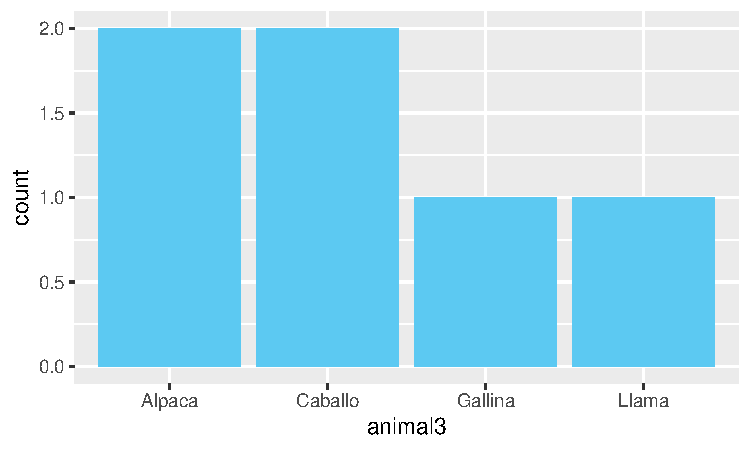
\includegraphics[width=\maxwidth]{figure/twenty_one-1} 
\end{knitrout}
	\caption{Animales al que se dedican las personas como tercera opcion}
	\end{figure}
	Se observa que la crianza a la que las personas se dedican como tercera opción es alpaca y Caballos en gran medida, seguida de Gallinas y Llama que se comportan en menor proporción.\\
	\\
	De la cantidad de animales que crian se tiene lo siguiente:
	\begin{figure}[H]
	\centering
\begin{knitrout}
\definecolor{shadecolor}{rgb}{0.969, 0.969, 0.969}\color{fgcolor}
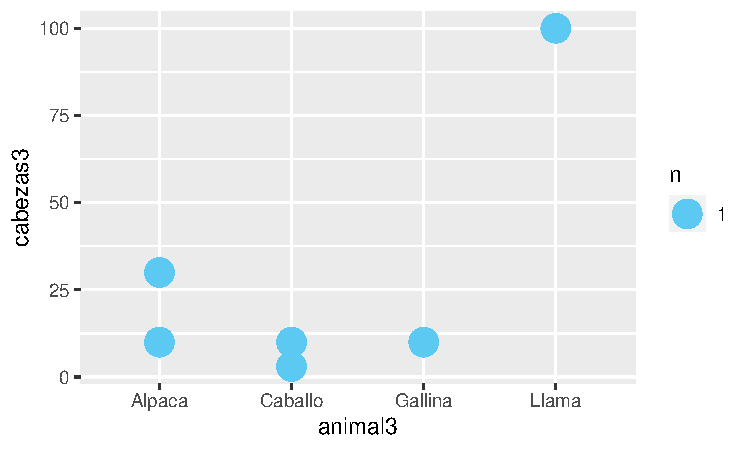
\includegraphics[width=\maxwidth]{figure/twenty_two-1} 
\end{knitrout}
	\caption{Cantidad de animales criados de tercera opcion en funcion a la cantidad y especie en \comunidad}
	\end{figure}
	Del gráfico se concluye que existen 100 llamas que crian como tercera opción en la comunidad de Chilloroya, seguido 30 alpacas, 15 gallinas y 10 caballos que tienen en su poder.\\
	\\
	Del metodo de crianza de esta opcion de animales se tiene lo siguiente:
	\begin{figure}[H]
	\centering
\begin{knitrout}
\definecolor{shadecolor}{rgb}{0.969, 0.969, 0.969}\color{fgcolor}
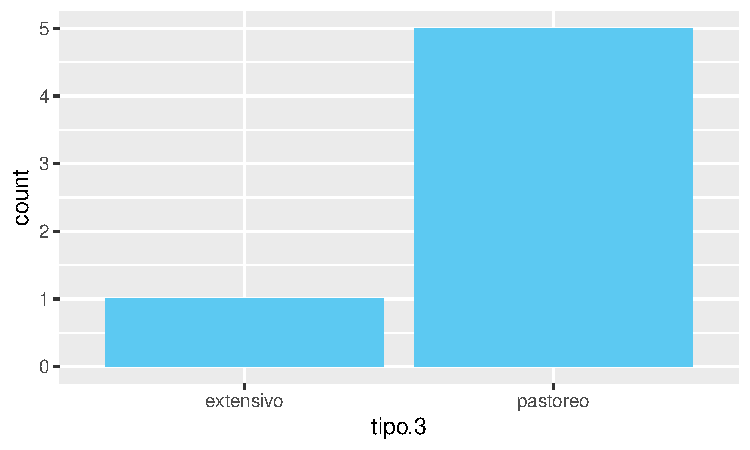
\includegraphics[width=\maxwidth]{figure/twenty_three-1} 
\end{knitrout}
	\caption{Metodo de crianza de la tercera opcion de crianza de animales en \comunidad}
	\end{figure}
	El método de crianza que tienen los pobladres a los animales de tercera opción, pricipalmente es el pastoreo en gran medida y el método extensivo en menor proporción.\\
	
	
	\section{Recurso hidrico}
	De las personas que acceden al servicio de las qochas se identifico que solo esta cantidad accede al servicio:
	\begin{figure}[H]
	\centering
\begin{knitrout}
\definecolor{shadecolor}{rgb}{0.969, 0.969, 0.969}\color{fgcolor}
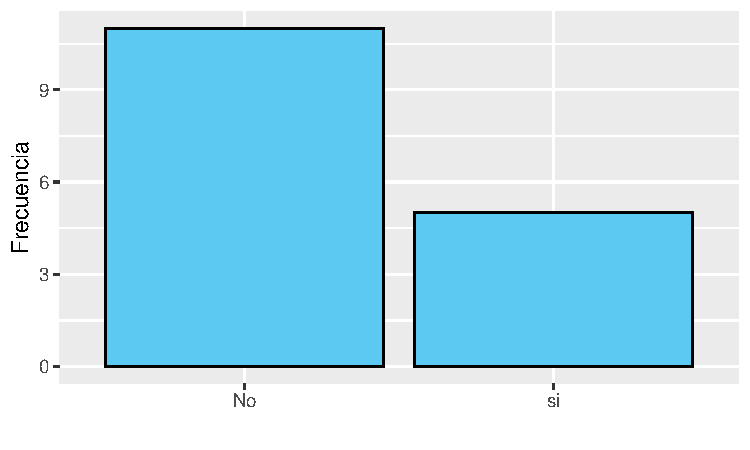
\includegraphics[width=\maxwidth]{figure/trece-1} 
\end{knitrout}
	\caption{Acceso al recurso}
	\end{figure}
	Se puede observar que la mayoria de los pobladores no acceden al recurso hídrico en la \comunidad, sin embargo en menor medida si.\\
	\\
	De los propietarios de la qocha se identifico las siguientes respuestas:
	\begin{figure}[H]
	\centering
\begin{knitrout}
\definecolor{shadecolor}{rgb}{0.969, 0.969, 0.969}\color{fgcolor}
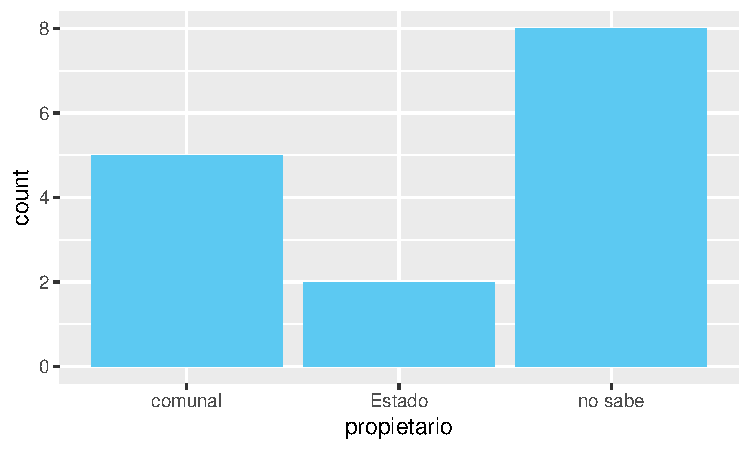
\includegraphics[width=\maxwidth]{figure/catorce-1} 
\end{knitrout}
	\caption{Propietario del recurso}
	\end{figure}
	Se identifica que la mayoria de los pobladores no saben si son propietarios de las qochas en consulta, un porcentaje menor afirman que las Qochas son de propiedad de la comunidad, finalmente reconocen como propietario al estado.\\
	\\
	Del uso que se da se tiene lo siguiente:
	\begin{figure}[H]
	\centering
\begin{knitrout}
\definecolor{shadecolor}{rgb}{0.969, 0.969, 0.969}\color{fgcolor}
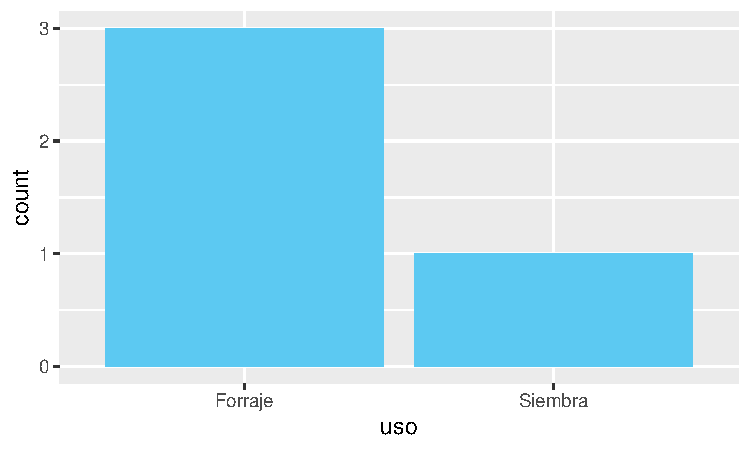
\includegraphics[width=\maxwidth]{figure/quince-1} 
\end{knitrout}
	\caption{Uso del recurso}
	\end{figure}
	De los pobladores que tienen acceso al uso del recursos, se identifico que todos lo utilizan para forraje y una parte utiliza para siembra.\\
	\\
	Se consulto si los beneficiarios estan satisfechos con el servicio de las qochas y se tuvo como resultado lo siguiente:
	\begin{figure}[H]
	\centering
\begin{knitrout}
\definecolor{shadecolor}{rgb}{0.969, 0.969, 0.969}\color{fgcolor}
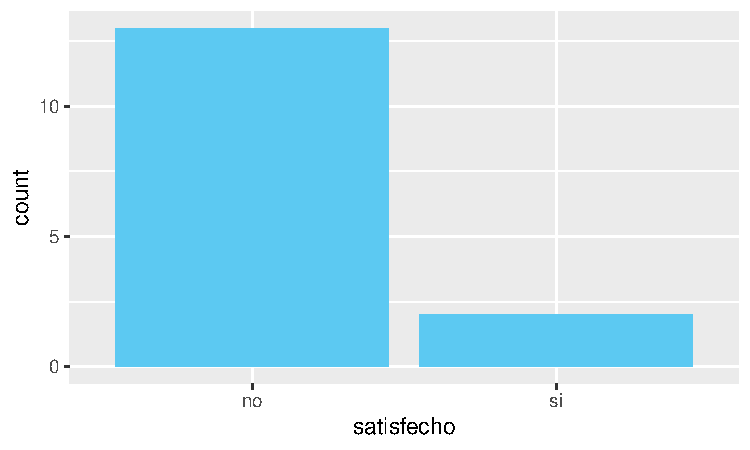
\includegraphics[width=\maxwidth]{figure/dieciseis-1} 
\end{knitrout}
	\caption{Satisfaccion con el uso del recurso}
	\end{figure}
	Como se puede observar, es mayor la población que no esta satisfecha con el uso del recurso hidríco en su comunidad, asu ves este no cuenta con un nivel adecuado para brindar el servicio. Finalmente hay un grupo pequeño que sí esta satisfecho con el recurso hídrico que recibe.\\
	\\
	Se consulto que otra fuente de agua usa en reemplazo del recurso, de los cual se tiene como resultado:
	\begin{figure}[H]
	\centering
\begin{knitrout}
\definecolor{shadecolor}{rgb}{0.969, 0.969, 0.969}\color{fgcolor}
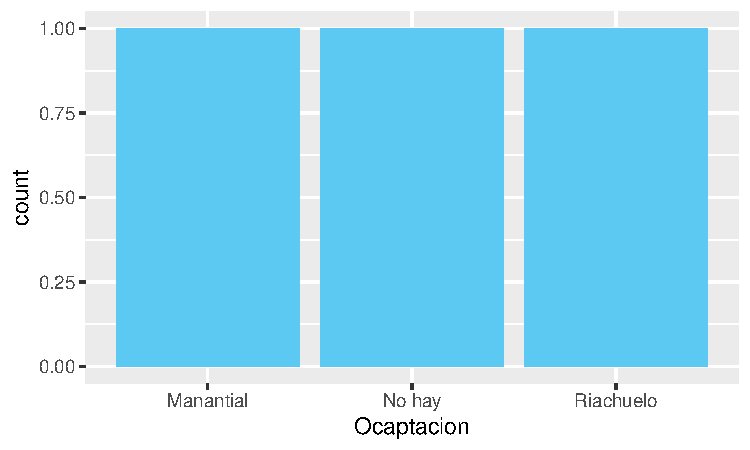
\includegraphics[width=\maxwidth]{figure/diecisiete-1} 
\end{knitrout}
	\caption{Otro recurso que suple la oferta del recurso}
	\end{figure}
	Se observa que el recurso que reemplaza es el manantial y riachuelo, siendo el segundo de mayor uso, finalmente se ha encontrado poblacion que no tiene acceso al recurso hídrio\\
	\\
	Se consulto cual es la razon por la que los usuarios no se sienten satisfechos y se identifico lo siguiente:
	\begin{figure}[H]
	\centering
\begin{knitrout}
\definecolor{shadecolor}{rgb}{0.969, 0.969, 0.969}\color{fgcolor}
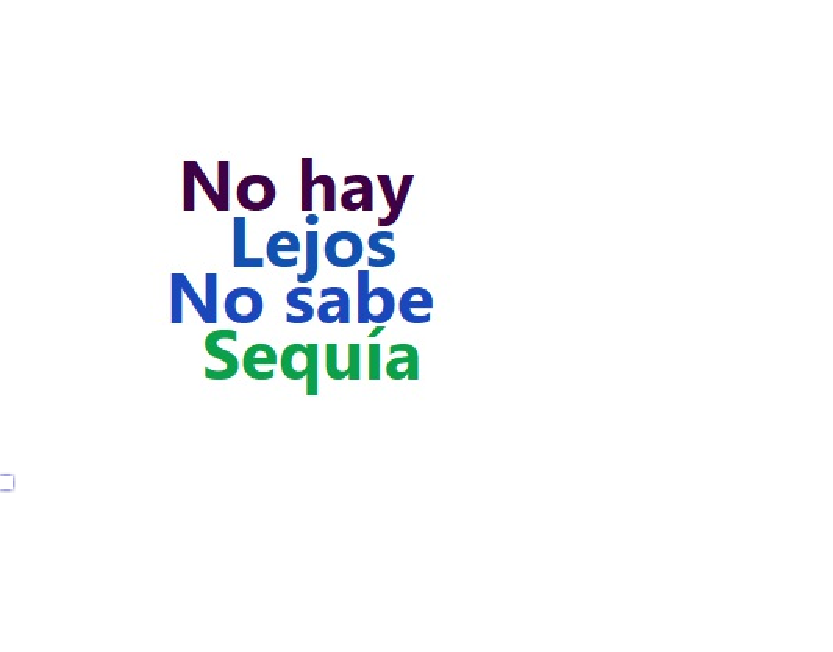
\includegraphics[width=\maxwidth]{figure/dieciocho-1} 
\end{knitrout}
	\caption{Razon de descontento}
	\end{figure}
	Debido a que las respuestas no son alternativas y son abiertas, se opto por utilizar mineria de datos para estas, de la cual se ha identificado que la opinion con mayor frecuencia es que el descontento se debe a la poca disponibilidad de agua o sequia.
	\section{Aspectos socioeconomicos}
	Se consulto cuantos integrantes de su familia trabajan, de lo cual se tiene la siguiente informacion
	\begin{figure}[H]
	\centering
\begin{knitrout}
\definecolor{shadecolor}{rgb}{0.969, 0.969, 0.969}\color{fgcolor}
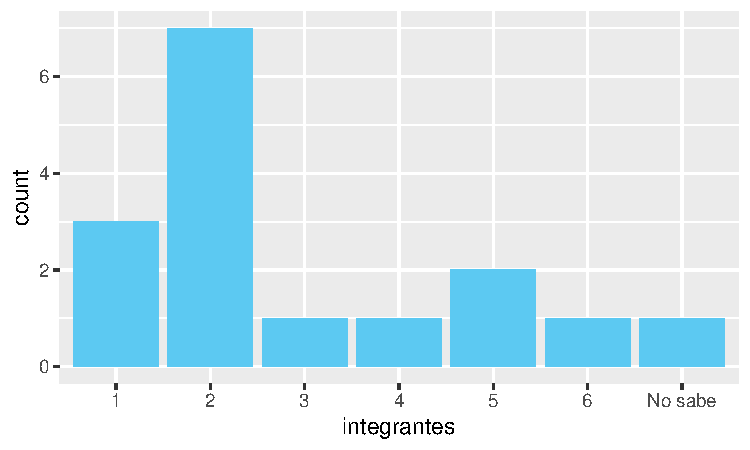
\includegraphics[width=\maxwidth]{figure/diecinueve-1} 
\end{knitrout}
	\caption{cantidad de integrantes que trabajan en la familia}
	\end{figure}
	Se observa que en la mayoria de familias trabajan con dos integrantes, seguido de un solo integrante que labora, sin embargo hay familias que trabajan con 5 integrantes, finalmente hay 3, 4 o 6 integrantes que trabajan en la familia\\
	\\
  Se consulto el ingreso familiar promedio de la familia de lo cual se tiene lo siguiente:
	\begin{figure}[H]
	\centering
\begin{knitrout}
\definecolor{shadecolor}{rgb}{0.969, 0.969, 0.969}\color{fgcolor}\begin{kframe}


{\ttfamily\noindent\color{warningcolor}{\#\# Warning: NAs introducidos por coerción}}\end{kframe}
\includegraphics[width=\maxwidth]{figure/veinte-1} 
\end{knitrout}
	\caption{Ingreso promedio de las familias de \comunidad}
	\end{figure}
	Se puede observar que el promedio de ingreso familiar en la comunidad de Chilloroya se sitúa entre 400 a 500 soles, seguido algunas familias tienen un ingreso que varia 400 a 950 soles, tambien se pudo obervar que el ingreso propmedio de la familia es de 3000 soles, finalmente se encontró que hay familias donde el ingreso varia entre 1000 a 1500 soles.\\
	\\
	Combinando la cantidad de integrantes que trabajan y el ingreso promedio mensual, se tiene lo siguiente:
	
	\begin{figure}[H]
	\centering
\begin{knitrout}
\definecolor{shadecolor}{rgb}{0.969, 0.969, 0.969}\color{fgcolor}\begin{kframe}


{\ttfamily\noindent\color{warningcolor}{\#\# Warning: NAs introducidos por coerción}}\end{kframe}
\includegraphics[width=\maxwidth]{figure/nose-1} 
\end{knitrout}
	\caption{Ingreso promedio de las familias de \comunidad en funciona a la cantidad de persionas que trabajan}
	\end{figure}
Los datos del gráfico muestra que 6 integrantes de la familia pueden generar un ingreso promedio mensual de 3000 soles, seguido de 2 integrantes que pueden generar un ingreso que varie de 500 a 1500 soles, tambien se observa que 5 integrantes tienen un promedio mensual que varia entre 600 a 700 soles.
	\section{Aspectos sociales y culturales}
	De la religion que los encuestados creen se tiene la siguiente informacion:
	\begin{figure}[H]
	\centering
\begin{knitrout}
\definecolor{shadecolor}{rgb}{0.969, 0.969, 0.969}\color{fgcolor}
\includegraphics[width=\maxwidth]{figure/veintiuno-1} 
\end{knitrout}
	\caption{Religion de los pobladores de \comunidad}
	\end{figure}
	Se puede observar que la mayoria de los encuestados es de religion católica, seguido de la religió Adventista, Israelita y  finalmente existen pobladores que pertenecen a ninguna religión.\\
	\\
	De la pregunta respecto a si alguna organización cultural se dedica a la realizacion de las actividades de las qochas
	\begin{figure}[H]
	\centering
\begin{knitrout}
\definecolor{shadecolor}{rgb}{0.969, 0.969, 0.969}\color{fgcolor}
\includegraphics[width=\maxwidth]{figure/veintidos-1} 
\end{knitrout}
	\caption{Organizacion dedicada a actividades culturales en la qocha}
	\end{figure}
	Se observa que la mayoria de los pobladores indica que no existe alguna organizacion dedicada a la realizacion de actividades culturales en la qocha, mientras que solo una persona indica que no sabe.  
	\section{Aspectos de gestion}
	De la consulta de la existencia de algun comite encargardo del funcionamiento de la qocha se obtuvo lo siguiente:
	\begin{figure}[H]
	\centering
\begin{knitrout}
\definecolor{shadecolor}{rgb}{0.969, 0.969, 0.969}\color{fgcolor}
\includegraphics[width=\maxwidth]{figure/veintitres-1} 
\end{knitrout}
	\caption{Comite encargado de la gestion del uso de la qocha en \comunidad}
	\end{figure}
	Se observa que la mayoria de los encuestados indican que no existe un comite de gestión encargado del uso de la qocha ademas un pequeño grupo señalan que si hay un comité.\\
	\\
	De la frecuencia al año con que se realizan actividades de mantenimiento o prevención
	\begin{figure}[H]
	\centering
\begin{knitrout}
\definecolor{shadecolor}{rgb}{0.969, 0.969, 0.969}\color{fgcolor}
\includegraphics[width=\maxwidth]{figure/veinticuatro-1} 
\end{knitrout}
	\caption{Frecuencia de realizacion de actividades de faena en la qocha}
	\end{figure}
	De la única persona que indica que existe un comite de gestión encargado de la qocha, se identifica que la frecuencia de realizacion de faenas es semestral, seguido del trimestral y anual.\\
	\\
	De la frecuencua, al año, con que se paga al comite se tiene la siguiente informacion:
	\begin{figure}[H]
	\centering
\begin{knitrout}
\definecolor{shadecolor}{rgb}{0.969, 0.969, 0.969}\color{fgcolor}
\includegraphics[width=\maxwidth]{figure/veinticinco-1} 
\end{knitrout}
	\caption{Pago realizado para el comite de gestion de qochas en \comunidad}
	\end{figure}
	De la unica persona que indica que existe un comite de gestión para las qochas, indica que no se realiza el pago a este comite.\\
	\\
	Existe alguna organizacion externa dedicada al cuidado de la qocha, de la cual se tiene la siguiente respuesta
	\begin{figure}[H]
	\centering
\begin{knitrout}
\definecolor{shadecolor}{rgb}{0.969, 0.969, 0.969}\color{fgcolor}
\includegraphics[width=\maxwidth]{figure/veintiseis-1} 
\end{knitrout}
	\caption{Organizacion externa encargada del cuidado de la qocha}
	\end{figure}
	Se observa que todos los encuestados indican que no existe una organización externa encargada del cuidado de qochas en \comunidad, solo un pequeño porcentaje de pobladores señalan que tienen cuidados a nivel externo.\\
	\\
	Se explicó informacion respecto a los beneficios del proyecto, por lo que se consulto si la persona estaria dispuesta en apoyar durante la fase de funcionamiento que comprende la operacion y mantenimiento, de lo cual se tiene la siguiente respuesta:
	\begin{figure}[H]
	\centering
\begin{knitrout}
\definecolor{shadecolor}{rgb}{0.969, 0.969, 0.969}\color{fgcolor}
\includegraphics[width=\maxwidth]{figure/veintisiete-1} 
\end{knitrout}
	\caption{Disposicion de apoyo durante la ejecucion del proyecto}
	\end{figure}
	Se observa que todos los encuestados estarian dispuestos a apoyar durante la fase de ejecucion del proyecto, en específico en la etapa operación y mantenimento de las presas o Qochas asimismo en las actividades que se intervenga con la parte agronómica en la comunidad.\\
	\\
	Explicada la constitucion de un comite encargado de la etapa de funcionamiento del proyecto se consulto la predisposicion de los encuestados a pagar una cuata maxima, de la cual se obtuvo las siguientes cantidades:
	\begin{figure}[H]
	\centering
\begin{knitrout}
\definecolor{shadecolor}{rgb}{0.969, 0.969, 0.969}\color{fgcolor}
\includegraphics[width=\maxwidth]{figure/veintiocho-1} 
\end{knitrout}
	\caption{Disposicion a pagar cuota durante el periodo de funcionamiento del proyecto}
	\end{figure}
	Se puede observar que entre quienes esten dispuestos a pagar y no, la proporción es muy cercana, siendo mas alta quienes si apoyarian a pagar, esto sugiere que los pobladores de la comuidad están comprometidos con la labor que vana a realizar despues ejecutado el proeyecto en la zona.\\
	\\
	De la consulta respecto a la percepcion de un adecuado uso de las qochas por parte de las personas, se tiene la siguiente informacion:
	\begin{figure}[H]
	\centering
\begin{knitrout}
\definecolor{shadecolor}{rgb}{0.969, 0.969, 0.969}\color{fgcolor}
\includegraphics[width=\maxwidth]{figure/veintinueve-1} 
\end{knitrout}
	\caption{Percepcion de uso adecuado de las qochas}
	En este caso las dos alternativas son muy cercanas en proporción, esto concluye que las Qochas son usadas en el riego de sus parcelas sí las condiciones geográficas lo permite, existe un porcentaje similar que no usan adecuadamente el agua de las Qochas.
	\end{figure}
	En este caso 
	\section{Aspectos de medio ambiente}
	Perjuicio en la actividad agropecuaria debido al cambio climatico
	\begin{figure}[H]
	\centering
\begin{knitrout}
\definecolor{shadecolor}{rgb}{0.969, 0.969, 0.969}\color{fgcolor}
\includegraphics[width=\maxwidth]{figure/treinta-1} 
\end{knitrout}
	\caption{Perjuicio en la actividad agropecuaria debido al cambio climatico}
	\end{figure}
	Como se aprecia los perjuicios producidos por el cambio climatico identificados por los encuestados son los siguientes: no hay nevados, poca agua, friaje y menor produccion.\\
	\\
	Especies de flora identificadas en la qocha
	
	\begin{figure}[H]
	\centering
\begin{knitrout}
\definecolor{shadecolor}{rgb}{0.969, 0.969, 0.969}\color{fgcolor}
\includegraphics[width=\maxwidth]{figure/treintayuno-1} 
\end{knitrout}
	\caption{Especies de flora identificadas en la qocha}
	\end{figure}
	Se puede observar que las especies de flora identificadas es Paja, Pasto natural, Paja brava  mientras que las demas son Paja, paja brava.\\
	\\
	Especies de fauna identificadas en la qocha
	\begin{figure}[H]
	
	\centering
\begin{knitrout}
\definecolor{shadecolor}{rgb}{0.969, 0.969, 0.969}\color{fgcolor}
\includegraphics[width=\maxwidth]{figure/treintaydos-1} 
\end{knitrout}
	\caption{Especies de fauna identificadas en la qocha}
	\end{figure}
	Se observa que la especie de fauna identificada con mayor frecuencia es Sapo, esto indica que el medio ambiente donde viven estas especies de anfibios están preservadas de una manera natural, no hay intervención química que alteren la vida. Finalmente no han identificado ninguna otra especie en la Qocha.\\
	\\
	Especies vegetales nativas en extincion.
	\begin{figure}[H]
	\centering
\begin{knitrout}
\definecolor{shadecolor}{rgb}{0.969, 0.969, 0.969}\color{fgcolor}
\includegraphics[width=\maxwidth]{figure/treintaytres-1} 
\end{knitrout}
	\caption{Especies vegetales en extincion}
	\end{figure}
	De las especies vegetales en peligrro de extincion, se ha identificado que el especie en peligro pérdida es el pasto, se podría concluir que el sobrepastoreo en la comunidad es la causa principal, así como tambien la escases del agua en la parte alta dificulta realizar activides de riego para estas especies. Seguido de las especies deOqoruro, Tacalafra escasean en la misma proporcion.\\
	\\
	Modificaciones identificadas en la turba de la qocha.
	\begin{figure}[H]
	\centering
\begin{knitrout}
\definecolor{shadecolor}{rgb}{0.969, 0.969, 0.969}\color{fgcolor}
\includegraphics[width=\maxwidth]{figure/treintaycuatro-1} 
\end{knitrout}
	\caption{Alteraciones de la turba en la qocha}
	\end{figure}
	Se observa que los pobladores identifican que la turba se esta secando y desapareciendo. Lo cual podría afirmar que hay pérdida de los factores que las mantiene como es el caso de a especies que habitan el lugar y el decaimiento de otras especies originales en el lugar\\
	\\
	Alteraciones en la precipitación pluvial en la zona de la qocha
	\begin{figure}[H]
	\centering
\begin{knitrout}
\definecolor{shadecolor}{rgb}{0.969, 0.969, 0.969}\color{fgcolor}
\includegraphics[width=\maxwidth]{figure/treintaycinco-1} 
\end{knitrout}
	\caption{Alteraciones pluviales en las zonas de qochas}
	\end{figure}
	La mayor alteracion pluvial que se ha indetificado es que hay menos lluvias en la zona de las qochas. \\
	\\
	Alteraciones en el suelo en la zona de la qocha
		\begin{figure}[H]
	\centering
\begin{knitrout}
\definecolor{shadecolor}{rgb}{0.969, 0.969, 0.969}\color{fgcolor}
\includegraphics[width=\maxwidth]{figure/treintayseis-1} 
\end{knitrout}
	\caption{Alteraciones en el suelo de las zonas de qochas}
	\end{figure}
	
	\begin{center}
		\textbf{Atentamente}
	\end{center}
	
	
	\begin{figure}[H]
		\centering
		\includegraphics[scale=0.35]{H:/Gore Cusco/img/firma}
	\end{figure}
	\thispagestyle{lastpage}




\end{document}
